\documentclass[11pt,a4paper]{article}
\usepackage[utf8]{inputenc}
\usepackage[T1]{fontenc}
\usepackage[polish]{babel}
\usepackage{lmodern}
\usepackage[margin=2.3cm]{geometry}
\usepackage{graphicx}
\usepackage{booktabs}
\usepackage{float}
\usepackage{caption}
\usepackage{amsmath}
\usepackage{microtype}
\usepackage[hidelinks]{hyperref}

\graphicspath{{../out/figures/}{zrzuty/}}
% Plik generowany przez raport/generuj_liczby.py - nie edytować ręcznie.
\newcommand{\nAll}{7200}
\newcommand{\nTrainDir}{5600}
\newcommand{\nTestDir}{1600}
\newcommand{\nAugTrain}{100}
\newcommand{\nAugTest}{103}
\newcommand{\nTrain}{5500}
\newcommand{\nTestDedup}{806}
\newcommand{\nDedupNotumor}{47}
\newcommand{\nMdGroups}{153}
\newcommand{\nMdFiles}{340}
\newcommand{\nPairs}{5893}
\newcommand{\nPairsConflict}{47}
\newcommand{\nPairsConflictGM}{39}
\newcommand{\leakZero}{370}
\newcommand{\leakZeroNotumor}{257}
\newcommand{\leakFour}{714}
\newcommand{\leakFourNotumor}{353}
\newcommand{\nGroups}{3928}
\newcommand{\nGroupsMax}{22}
\newcommand{\nGroupsSingle}{3165}
\newcommand{\nResolutions}{447}
\newcommand{\fracFiveNotumor}{1,1\,\%}
\newcommand{\fracFiveTumorMin}{86\,\%}
\newcommand{\meanIntGlioma}{33,1}
\newcommand{\meanIntNotumor}{61,7}
\newcommand{\nTrainMeningioma}{1300}
\newcommand{\cvFCnn}{0,955}
\newcommand{\cvFsdCnn}{0,006}
\newcommand{\cvAccCnn}{0,955}
\newcommand{\cvSecCnn}{11}
\newcommand{\cvParamsCnn}{1,2}
\newcommand{\cvBestEpochCnn}{28}
\newcommand{\cvFEff}{0,981}
\newcommand{\cvFsdEff}{0,006}
\newcommand{\cvAccEff}{0,981}
\newcommand{\cvSecEff}{6}
\newcommand{\cvParamsEff}{4,0}
\newcommand{\cvBestEpochEff}{12}
\newcommand{\cvFRes}{0,984}
\newcommand{\cvFsdRes}{0,005}
\newcommand{\cvAccRes}{0,984}
\newcommand{\cvSecRes}{11}
\newcommand{\cvParamsRes}{23,5}
\newcommand{\cvBestEpochRes}{9}
\newcommand{\cvFResTuned}{0,987}
\newcommand{\cvFsdResTuned}{0,006}
\newcommand{\cvAccResTuned}{0,987}
\newcommand{\cvSecResTuned}{13}
\newcommand{\cvParamsResTuned}{23,5}
\newcommand{\cvBestEpochResTuned}{12}
\newcommand{\nTrials}{20}
\newcommand{\nTrialsFail}{1}
\newcommand{\nTrialsComplete}{14}
\newcommand{\nTrialsPruned}{6}
\newcommand{\optBest}{0,992}
\newcommand{\optWorst}{0,956}
\newcommand{\optLr}{2,24\cdot 10^{-3}}
\newcommand{\optWd}{1,48\cdot 10^{-3}}
\newcommand{\optDropout}{0,12}
\newcommand{\optBatch}{16}
\newcommand{\optUnfreeze}{3}
\newcommand{\nBlocks}{5}
\newcommand{\accTestCnn}{0,919}
\newcommand{\accCiTestCnn}{0,906--0,932}
\newcommand{\fTestCnn}{0,918}
\newcommand{\fCiTestCnn}{0,904--0,930}
\newcommand{\aucTestCnn}{0,974}
\newcommand{\eceTestCnn}{0,031}
\newcommand{\accDedupCnn}{0,872}
\newcommand{\accCiDedupCnn}{0,850--0,895}
\newcommand{\fDedupCnn}{0,822}
\newcommand{\fCiDedupCnn}{0,790--0,853}
\newcommand{\aucDedupCnn}{0,963}
\newcommand{\eceDedupCnn}{0,070}
\newcommand{\accTestEff}{0,953}
\newcommand{\accCiTestEff}{0,943--0,963}
\newcommand{\fTestEff}{0,952}
\newcommand{\fCiTestEff}{0,941--0,962}
\newcommand{\aucTestEff}{0,993}
\newcommand{\eceTestEff}{0,036}
\newcommand{\accDedupEff}{0,914}
\newcommand{\accCiDedupEff}{0,896--0,933}
\newcommand{\fDedupEff}{0,874}
\newcommand{\fCiDedupEff}{0,843--0,900}
\newcommand{\aucDedupEff}{0,990}
\newcommand{\eceDedupEff}{0,067}
\newcommand{\accTestRes}{0,949}
\newcommand{\accCiTestRes}{0,938--0,959}
\newcommand{\fTestRes}{0,948}
\newcommand{\fCiTestRes}{0,936--0,958}
\newcommand{\aucTestRes}{0,991}
\newcommand{\eceTestRes}{0,040}
\newcommand{\accDedupRes}{0,906}
\newcommand{\accCiDedupRes}{0,886--0,926}
\newcommand{\fDedupRes}{0,866}
\newcommand{\fCiDedupRes}{0,834--0,893}
\newcommand{\aucDedupRes}{0,987}
\newcommand{\eceDedupRes}{0,077}
\newcommand{\accTestResTuned}{0,957}
\newcommand{\accCiTestResTuned}{0,946--0,966}
\newcommand{\fTestResTuned}{0,956}
\newcommand{\fCiTestResTuned}{0,945--0,965}
\newcommand{\aucTestResTuned}{0,989}
\newcommand{\eceTestResTuned}{0,036}
\newcommand{\accDedupResTuned}{0,917}
\newcommand{\accCiDedupResTuned}{0,898--0,935}
\newcommand{\fDedupResTuned}{0,886}
\newcommand{\fCiDedupResTuned}{0,857--0,913}
\newcommand{\aucDedupResTuned}{0,986}
\newcommand{\eceDedupResTuned}{0,071}
\newcommand{\sensTestGlioma}{0,833}
\newcommand{\sensCiTestGlioma}{0,792--0,866}
\newcommand{\specTestGlioma}{1,000}
\newcommand{\specCiTestGlioma}{1,000--1,000}
\newcommand{\aucTestGlioma}{0,965}
\newcommand{\sensTestMeningioma}{0,995}
\newcommand{\sensCiTestMeningioma}{0,987--1,000}
\newcommand{\specTestMeningioma}{0,965}
\newcommand{\specCiTestMeningioma}{0,954--0,975}
\newcommand{\aucTestMeningioma}{0,992}
\newcommand{\sensTestNotumor}{1,000}
\newcommand{\sensCiTestNotumor}{1,000--1,000}
\newcommand{\specTestNotumor}{0,979}
\newcommand{\specCiTestNotumor}{0,971--0,987}
\newcommand{\aucTestNotumor}{0,999}
\newcommand{\sensTestPituitary}{1,000}
\newcommand{\sensCiTestPituitary}{1,000--1,000}
\newcommand{\specTestPituitary}{0,998}
\newcommand{\specCiTestPituitary}{0,996--1,000}
\newcommand{\aucTestPituitary}{1,000}
\newcommand{\sensDedupGlioma}{0,793}
\newcommand{\sensCiDedupGlioma}{0,748--0,837}
\newcommand{\specDedupGlioma}{1,000}
\newcommand{\specCiDedupGlioma}{1,000--1,000}
\newcommand{\aucDedupGlioma}{0,958}
\newcommand{\sensDedupMeningioma}{0,986}
\newcommand{\sensCiDedupMeningioma}{0,965--1,000}
\newcommand{\specDedupMeningioma}{0,939}
\newcommand{\specCiDedupMeningioma}{0,920--0,957}
\newcommand{\aucDedupMeningioma}{0,986}
\newcommand{\sensDedupNotumor}{1,000}
\newcommand{\sensCiDedupNotumor}{1,000--1,000}
\newcommand{\specDedupNotumor}{0,967}
\newcommand{\specCiDedupNotumor}{0,954--0,979}
\newcommand{\aucDedupNotumor}{0,998}
\newcommand{\sensDedupPituitary}{1,000}
\newcommand{\sensCiDedupPituitary}{1,000--1,000}
\newcommand{\specDedupPituitary}{0,996}
\newcommand{\specCiDedupPituitary}{0,990--1,000}
\newcommand{\aucDedupPituitary}{1,000}
\newcommand{\nErrTest}{69}
\newcommand{\nErrDedup}{67}
\newcommand{\nErrGM}{42}
\newcommand{\fracErrGM}{61\,\%}
\newcommand{\errRateTwin}{0,0\,\%}
\newcommand{\errRateNoTwin}{7,6\,\%}
\newcommand{\camBg}{15,6\,\%}
\newcommand{\camBgArea}{43,8\,\%}
\newcommand{\camBorder}{11,2\,\%}
\newcommand{\camBgNotumor}{36,6\,\%}
\newcommand{\camBgOk}{15,4\,\%}
\newcommand{\camBgErr}{17,4\,\%}
\newcommand{\gliomaOtherTrain}{0}
\newcommand{\gliomaOtherTest}{76}
\newcommand{\gliomaOtherErr}{66}
\newcommand{\gliomaFiveTest}{324}
\newcommand{\gliomaFiveErr}{1}
\newcommand{\gliomaOtherErrRate}{86,8\,\%}
\newcommand{\notumorOtherTrain}{1383}
\newcommand{\meningiomaOtherTrain}{133}
\newcommand{\nErrGliomaNotumor}{25}
\newcommand{\nErrGliomaMeningioma}{42}
\newcommand{\nErrGlioma}{67}
\newcommand{\camBgTumor}{14,3\,\%}
\newcommand{\camBorderNotumor}{23,8\,\%}
\newcommand{\camBorderTumor}{10,4\,\%}
\newcommand{\borderArea}{35\,\%}
\newcommand{\impLr}{0,61}
\newcommand{\impDropout}{0,29}
\newcommand{\impWd}{0,09}

\newcommand{\tabela}[1]{\input{tabele/#1.tex}}

\begin{document}

% ---------------------------------------------------------------- strona tytułowa
\pagenumbering{Alph}
\begin{titlepage}
\centering
{\Large Politechnika Krakowska\par}
\vspace{2mm}
{\large Wydział Informatyki i Telekomunikacji\par}
\vspace{2mm}
{\large Studia Stacjonarne\par}
\vspace{4cm}
{\large Sprawozdanie z przedmiotu:\par}
\vspace{2mm}
{\LARGE\bfseries Uczenie Maszynowe w Diagnostyce Medycznej\par}
\vspace{2cm}
{\large Temat Projektu:\par}
\vspace{2mm}
{\Large Klasyfikacja guzów mózgu na obrazach rezonansu magnetycznego\par}
\vfill
\begin{flushright}
{\large Wykonał:\par}
{\large Jakub Balicki\par}
\end{flushright}
\vspace{1cm}
{\large Kraków, \today\par}
\end{titlepage}
\pagenumbering{arabic}

\tableofcontents
\newpage

% ---------------------------------------------------------------- 1
\section{Wstęp}

\subsection*{Cel projektu}
Celem projektu jest automatyczna klasyfikacja pojedynczych przekrojów MRI mózgu do jednej
z czterech klas: glejak (\texttt{glioma}), oponiak (\texttt{meningioma}), guz przysadki
(\texttt{pituitary}) oraz brak guza (\texttt{notumor}). Taki klasyfikator mógłby wspierać
wstępną selekcję badań (triage), np. wskazywać radiologowi badania z podejrzeniem guza.
Z punktu widzenia klinicznego najważniejsze jest, żeby nie przeoczyć guza (czułość dla klas
nowotworowych, swoistość dla klasy \texttt{notumor}) oraz żeby rzetelnie ocenić, na ile
wynik przeniesie się na nowych pacjentów.

\subsection*{Opis danych}
Wykorzystano publiczny zbiór \emph{Brain Tumor MRI Dataset} (M.~Nickparvar, Kaggle), który
łączy kilka źródeł: figshare, SARTAJ i Br35H. Pobrana wersja zawiera \nAll{} obrazów JPG
w skali szarości: \nTrainDir{} w katalogu \texttt{Training} i \nTestDir{} w~\texttt{Testing},
po równo w każdej klasie (tab.~\ref{tab:dane}). Cechy to piksele obrazu; nie ma żadnych
metadanych (wieku, płci, identyfikatora pacjenta ani rodzaju sekwencji).

Kontrola jakości (rozdz.~\ref{sec:eda}) ujawniła kilka problemów:
\begin{itemize}
\item balans klas jest sztuczny: klasę \texttt{meningioma} dopełniono \nAugTrain{}~+~\nAugTest{}
  przekształconymi kopiami istniejących obrazów (pliki \texttt{*-aug-me\_*}), a starsze opisy
  zbioru podają 7023 obrazy o innych licznościach klas,
\item \nMdGroups{} grup identycznych plików (\nMdFiles{} plików) oraz \nPairs{} par niemal identycznych
  obrazów; \leakFour{} z \nTestDir{} obrazów testowych ma bliźniaka w zbiorze treningowym,
\item \nPairsConflict{} par niemal identycznych obrazów ma różne etykiety (głównie glejak/oponiak),
\item klasy pochodzą z różnych źródeł: obrazy z guzami to prawie wyłącznie 512$\times$512 i T1 po
  kontraście, obrazy \texttt{notumor} mają różne rozdzielczości i sekwencje.
\end{itemize}

\begin{table}[H]
\centering
\caption{Liczność klas. ,,aug'' -- sztuczne kopie; ,,trening'' -- zbiór używany do uczenia
(bez kopii); \texttt{test\_dedup} -- test oczyszczony z duplikatów treningu (rozdz.~\ref{sec:dup}).}
\label{tab:dane}
\tabela{dane}
\end{table}

\subsection*{Zakres projektu}
Zrealizowano: eksploracyjną analizę danych z kontrolą duplikatów i wycieku, walidację
krzyżową z grupowaniem duplikatów, porównanie trzech modeli (CNN uczona od zera,
EfficientNetB0 i ResNet50 z transferem wiedzy), strojenie hiperparametrów biblioteką Optuna,
jednorazową ewaluację na zbiorze testowym z metrykami klinicznymi i przedziałami ufności,
kalibrację, wyjaśnialność metodą Grad-CAM, analizę błędów oraz prosty interfejs graficzny
w Streamlit. Kod jest w repozytorium (rozdz.~\ref{sec:zal}); każda liczba w raporcie jest
generowana skryptem \texttt{raport/generuj\_liczby.py} z plików w \texttt{out/metrics/}.

% ---------------------------------------------------------------- 2
\section{Przygotowanie danych}

\subsection*{Eksploracyjna analiza danych (EDA)}\label{sec:eda}
Notatnik \texttt{01\_eda.ipynb}. Przykładowe obrazy przedstawia rys.~\ref{fig:przyklady}.
W każdej klasie są przekroje w trzech płaszczyznach (osiowej, czołowej, strzałkowej).

\begin{figure}[H]
\centering
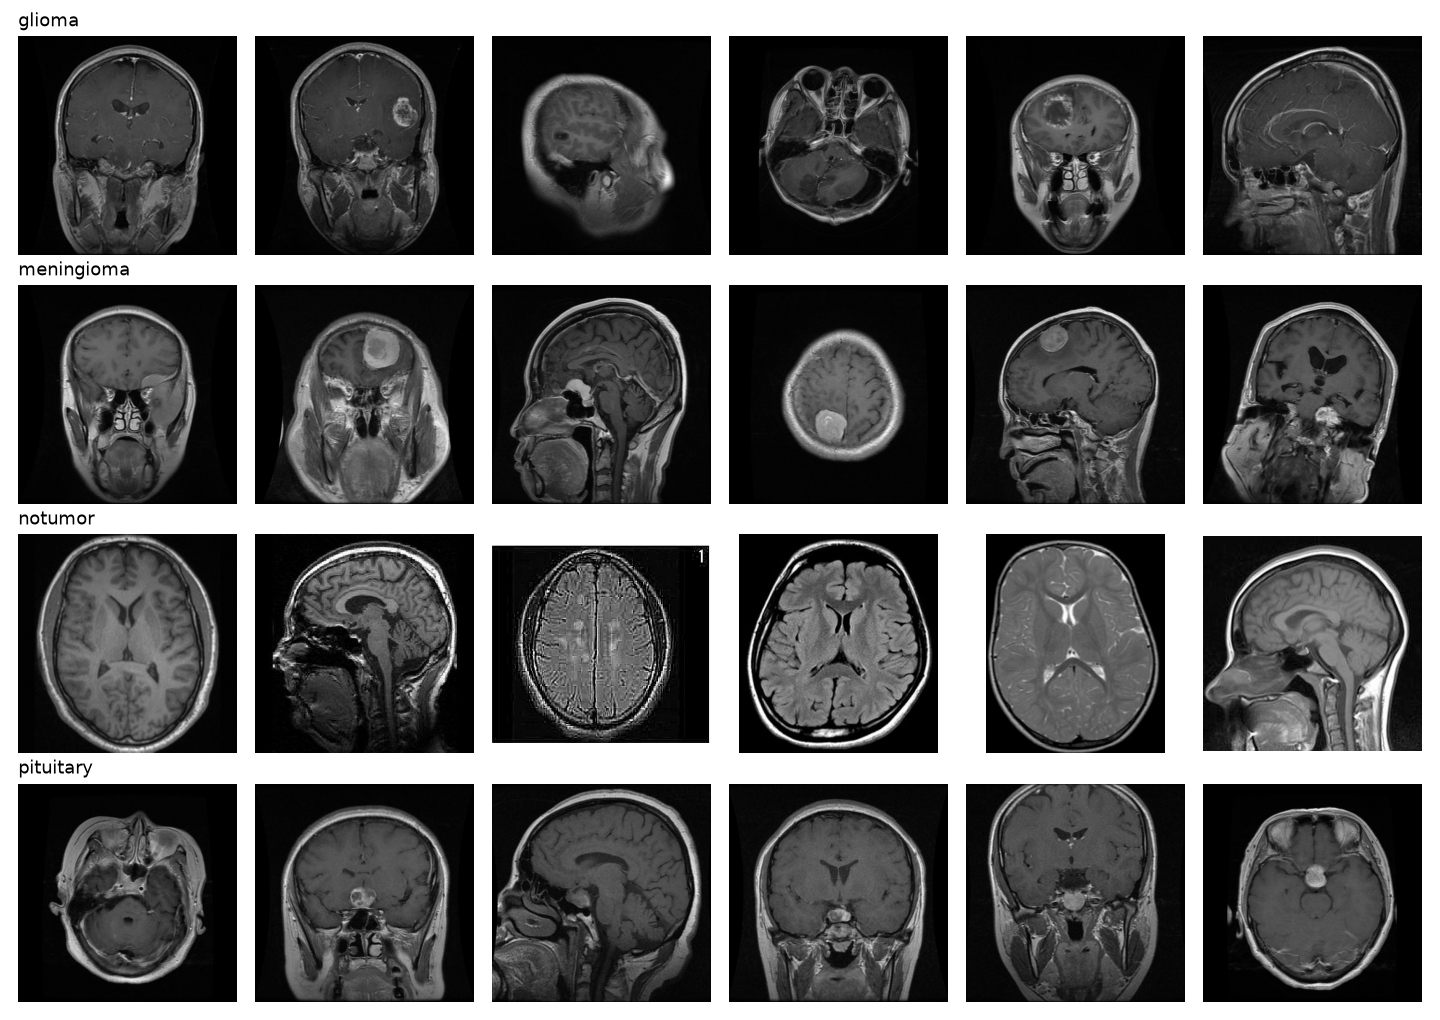
\includegraphics[width=0.9\linewidth]{eda_przyklady.png}
\caption{Losowe obrazy treningowe z każdej klasy.}
\label{fig:przyklady}
\end{figure}

\paragraph{Rozdzielczość i kanały.} Obrazy mają \nResolutions{} różnych rozdzielczości. Co najmniej
\fracFiveTumorMin{} obrazów w każdej z klas z guzem ma 512$\times$512 pikseli, a w klasie
\texttt{notumor} tylko \fracFiveNotumor{}. Pliki są zapisane jako skala szarości lub RGB, ale
w RGB kanały są praktycznie identyczne, więc wszystkie obrazy zamieniamy na jeden kanał szarości.

\paragraph{Jasność.} Średnia jasność obrazów różni się między klasami
(rys.~\ref{fig:jasnosc}): obrazy glejaków są najciemniejsze (średnio \meanIntGlioma{} w skali
0--255), obrazy bez guza -- najjaśniejsze (\meanIntNotumor{}).
Guz zajmuje mały fragment obrazu, więc różnica wynika głównie ze sposobu akwizycji
(sekwencja, okno wyświetlania, źródło danych). Istnieje więc ryzyko, że model nauczy się
rozpoznawać \emph{źródło} lub \emph{kontrast} obrazu zamiast guza -- sprawdzamy to w rozdz.~\ref{sec:xai}.

\begin{figure}[H]
\centering
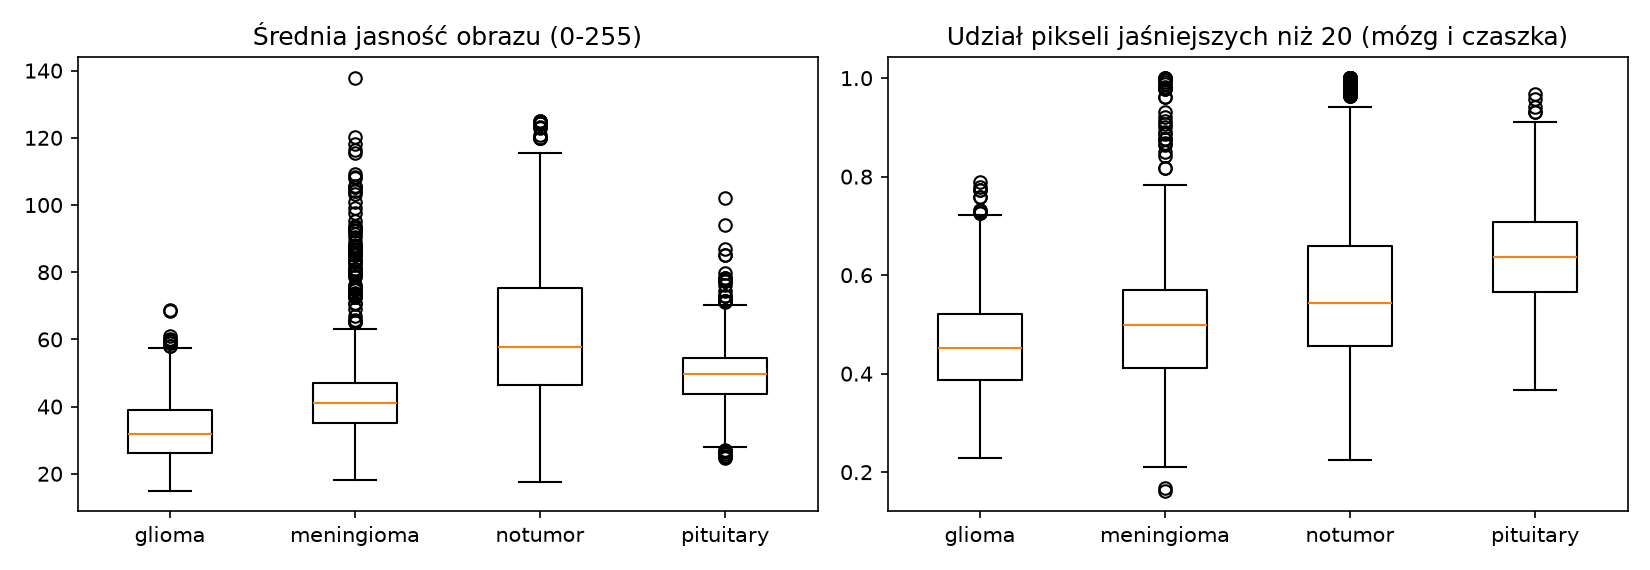
\includegraphics[width=0.85\linewidth]{eda_jasnosc.png}
\caption{Średnia jasność obrazu i udział pikseli nie-tła w klasach (zbiór treningowy).}
\label{fig:jasnosc}
\end{figure}

\paragraph{Duplikaty i wyciek.}\label{sec:dup}
Zbiór nie zawiera identyfikatora pacjenta, więc nie da się zastosować podziału per pacjent
(Leave-One-Group-Out). Zamiast tego szukaliśmy obrazów identycznych (skrót MD5 pliku)
i niemal identycznych (perceptual hash, pHash: 64-bitowy skrót z transformaty DCT obrazu
32$\times$32; odległość Hamminga między skrótami mierzy podobieństwo). Po obejrzeniu par
o różnych odległościach (rys.~\ref{fig:pary}) przyjęliśmy próg 4~bitów: przy 0--2 są to te
same obrazy (czasem inaczej przycięte), przy~4 ten sam lub sąsiedni przekrój tego samego
badania, przy 6 i więcej coraz częściej różne osoby. Tabela~\ref{tab:wyciek} pokazuje, że
nawet przy progu~0 aż \leakZero{} obrazów testowych (w tym \leakZeroNotumor{} z klasy
\texttt{notumor}) ma kopię w treningu; przy progu~4 jest ich \leakFour{} (\leakFourNotumor{}
z 400 obrazów \texttt{notumor}). Wynik na oryginalnym teście jest więc częściowo
,,sprawdzaniem pamięci'' modelu.

\begin{figure}[H]
\centering
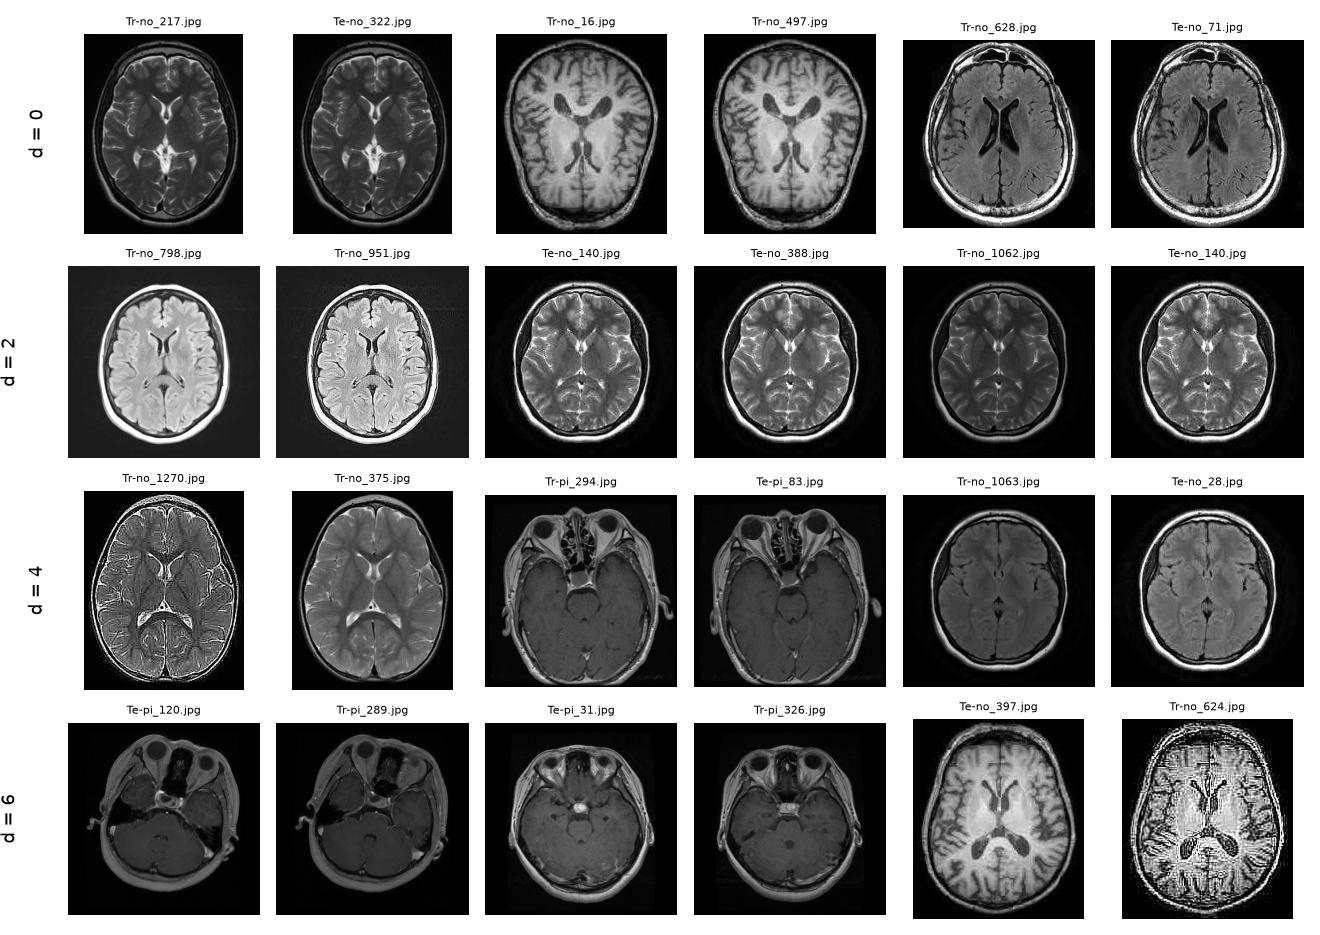
\includegraphics[width=0.85\linewidth]{eda_pary_phash.png}
\caption{Losowe pary obrazów o odległości Hamminga pHash $d = 0, 2, 4, 6$ (wiersze).}
\label{fig:pary}
\end{figure}

\begin{table}[H]
\centering
\caption{Liczba obrazów testowych, które mają w treningu obraz o odległości pHash nie większej niż próg.}
\label{tab:wyciek}
\tabela{wyciek}
\end{table}

Wśród par niemal-duplikatów \nPairsConflict{} ma różne etykiety, z czego \nPairsConflictGM{}
to pary glejak--oponiak (rys.~\ref{fig:konflikty}). Jest to szum etykiet, który ogranicza
osiągalną dokładność dla tych dwóch klas. Pliki \texttt{aug} okazały się odbitymi lub
obróconymi kopiami oryginalnych oponiaków -- także z drugiego katalogu (część kopii
w teście pochodzi od obrazów treningowych).

\begin{figure}[H]
\centering
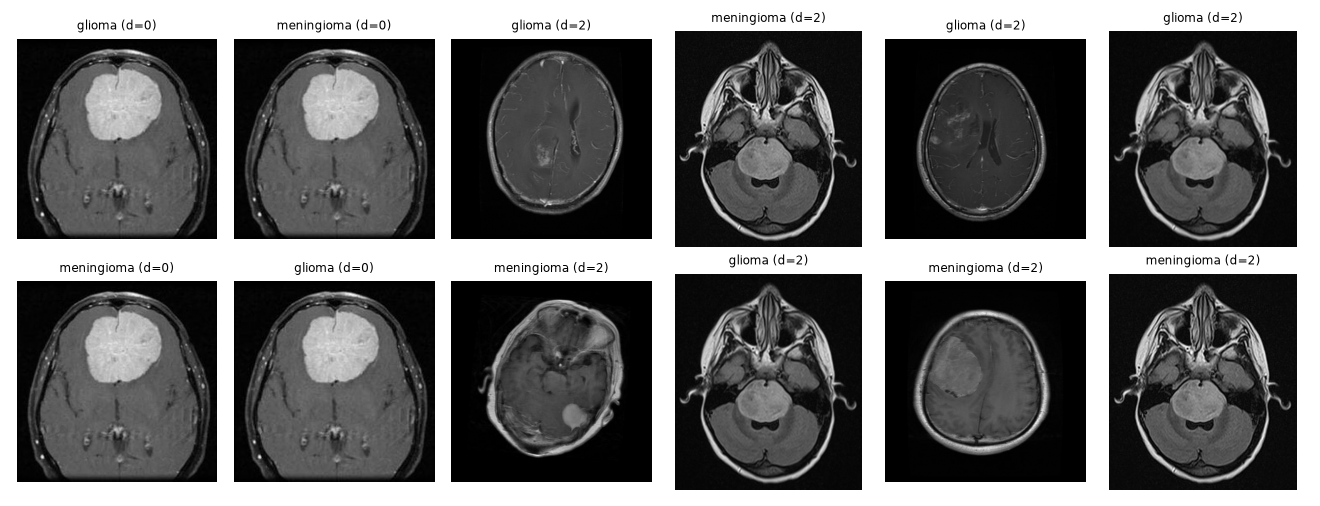
\includegraphics[width=0.85\linewidth]{eda_konflikty_etykiet.png}
\caption{Pary niemal identycznych obrazów z różnymi etykietami (górny i dolny wiersz to para).}
\label{fig:konflikty}
\end{figure}

\subsection*{Przetwarzanie danych}
\begin{itemize}
\item Odrzucenie sztucznych kopii \texttt{aug}; zbiór treningowy liczy \nTrain{} obrazów
  (\nTrainMeningioma{} oponiaków i po 1400 obrazów pozostałych klas). Niewielka nierównowaga nie wymagała wag klas
  ani oversamplingu.
\item Zbiór testowy oczyszczony (\texttt{test\_dedup}, \nTestDedup{} obrazów): bez obrazów
  z bliźniakiem w treningu i bez kopii \texttt{aug}. Wyniki raportujemy na obu wersjach testu.
\item Konwersja do skali szarości i skalowanie do 224$\times$224 (interpolacja dwuliniowa).
  Normalizacja: dla CNN od zera -- średnią i odchyleniem jasności zbioru treningowego (stałe w \texttt{src/models.py}),
  dla sieci z ImageNet -- kopiowanie kanału na 3 i statystyki ImageNet.
\item Augmentacja zgodna z domeną MRI: odbicie w poziomie (mózg jest w przybliżeniu
  symetryczny, a guz może wystąpić po każdej stronie), obrót do $\pm$10°, przesunięcie do 5\,\%,
  skalowanie 0,9--1,1. Celowo \emph{bez} zmian jasności i kontrastu: intensywność sygnału MRI
  niesie informację diagnostyczną, a różnice jasności między klasami chcieliśmy zbadać,
  a nie zamaskować.
\item Grupy niemal-duplikatów w treningu (\nGroups{} grup, największa ma \nGroupsMax{} obrazów)
  wykorzystano w walidacji krzyżowej (rozdz.~\ref{sec:trening}).
\end{itemize}

% ---------------------------------------------------------------- 3
\section{Modelowanie i ewaluacja}
\subsection*{Wybór modeli}
Porównano trzy sieci konwolucyjne (kod: \texttt{src/models.py}):
\begin{enumerate}
\item \textbf{CNN uczona od zera} (\cvParamsCnn{} mln parametrów): 4 bloki
  [Conv 3$\times$3 -- BatchNorm -- ReLU]$\times$2 + MaxPool (32--256 filtrów), globalne
  uśrednianie, dropout i warstwa liniowa. Punkt odniesienia, który pokazuje, ile daje
  transfer wiedzy.
\item \textbf{EfficientNetB0} (\cvParamsEff{} mln parametrów) z wagami ImageNet: mała sieć
  o dobrym stosunku dokładności do rozmiaru, odpowiednia do wdrożenia na zwykłym komputerze.
\item \textbf{ResNet50} (\cvParamsRes{} mln parametrów) z wagami ImageNet: klasyczna, większa
  sieć z połączeniami rezydualnymi, często stosowana jako punkt odniesienia w obrazowaniu medycznym.
\end{enumerate}
Modele klasyczne (np. regresja logistyczna, SVM, lasy losowe) wymagałyby ręcznego
wyznaczania cech z obrazu. Przy kilku tysiącach obrazów sieci konwolucyjne z transferem
wiedzy są standardowym i skuteczniejszym wyborem. Transfer learning przebiegał dwuetapowo.
Przez pierwsze 2 epoki szkielet był zamrożony i uczyła się tylko nowa głowica. Potem
odmrażano ostatnie bloki szkieletu (EfficientNetB0: 4 z 9, ResNet50: \texttt{layer3}
i \texttt{layer4}) z LR 10 razy mniejszym niż głowica, żeby nie zniszczyć wag z ImageNet.

\subsection*{Proces trenowania}\label{sec:trening}
\begin{itemize}
\item \textbf{Podział.} Test = katalog \texttt{Testing}, użyty jeden raz na końcu
  (skrypt \texttt{src/evaluate.py}); żadna decyzja nie była podejmowana na jego podstawie.
  Na \nTrain{} obrazach treningowych: \textbf{Stratified Group K-Fold, $K=5$}. Stratyfikacja
  zachowuje proporcje klas w foldach, a grupy niemal-duplikatów (\nGroups{} grup) nigdy nie są
  rozdzielane między trening i walidację foldu. Jest to przybliżenie walidacji grupowej
  (Leave-One-Group-Out) z wykładu, skoro zbiór nie ma identyfikatora pacjenta.
\item \textbf{Uczenie.} AdamW, entropia krzyżowa, kosinusowy harmonogram LR, mieszana precyzja
  bf16, stałe ziarno losowania. CNN: 30 epok, sieci z ImageNet: 15 epok. Po każdej epoce
  liczono macro-F1 na walidacji i zapamiętywano wagi \emph{najlepszej} epoki.
\item \textbf{Model końcowy.} Każda architektura została ponownie wytrenowana na całym zbiorze
  treningowym przez tę samą liczbę epok co w CV. Krzywe walidacyjne
  (rys.~\ref{fig:krzywe}) są pod koniec harmonogramu płaskie, a mediana najlepszej epoki to
  \cvBestEpochCnn{}/30 (CNN), \cvBestEpochEff{}/15 (EfficientNetB0) i \cvBestEpochRes{}/15
  (ResNet50), więc ostatnia epoka jest bliska najlepszej.
\item \textbf{Oversampling} nie był potrzebny: po odrzuceniu kopii \texttt{aug} klasy liczą
  \nTrainMeningioma{}--1400 obrazów.
\end{itemize}

\begin{figure}[H]
\centering
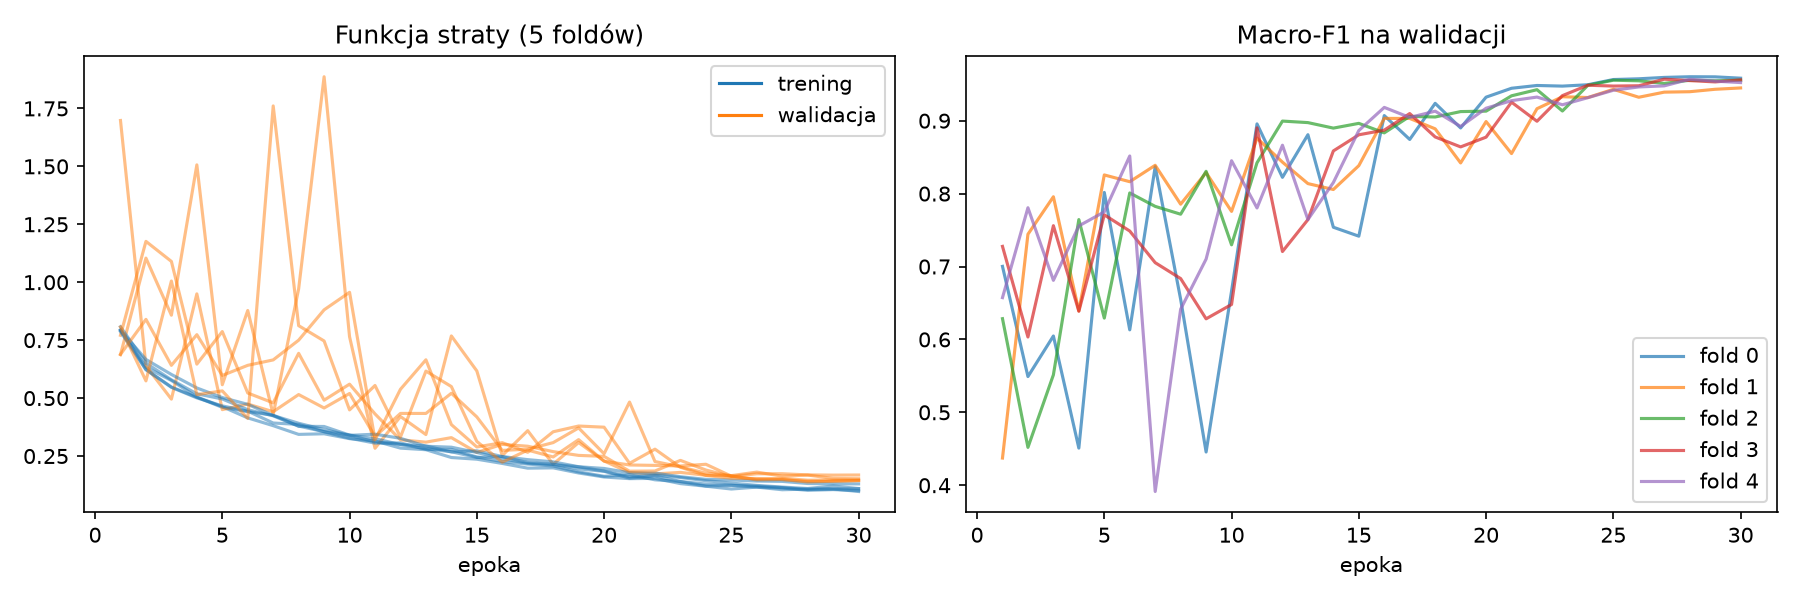
\includegraphics[width=\linewidth]{cv_cnn_krzywe.png}
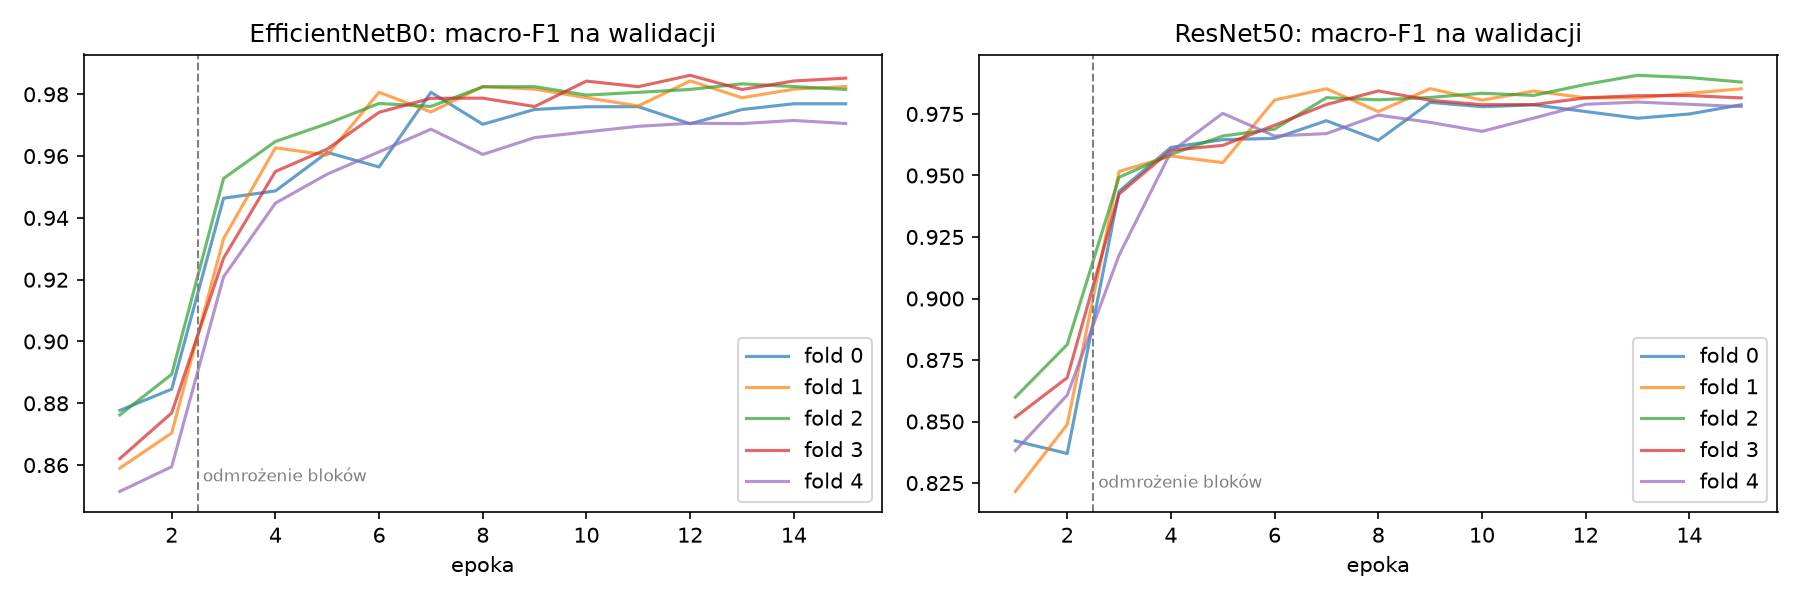
\includegraphics[width=\linewidth]{cv_transfer_krzywe.png}
\caption{Krzywe uczenia w 5 foldach: CNN od zera (góra) oraz macro-F1 na walidacji dla
EfficientNetB0 i ResNet50 (dół). Linia przerywana -- odmrożenie bloków szkieletu.}
\label{fig:krzywe}
\end{figure}

\subsection*{Ewaluacja}
Metryki (\texttt{src/metrics.py}) liczone w układzie ,,klasa kontra reszta'':
\begin{itemize}
\item \textbf{czułość} (recall) $= TP/(TP+FN)$ -- jaki odsetek obrazów danej klasy model wykrył,
\item \textbf{swoistość} $= TN/(TN+FP)$ -- jaki odsetek obrazów innych klas model poprawnie
  do tej klasy nie przypisał,
\item \textbf{precyzja} $= TP/(TP+FP)$, \textbf{F1} (średnia harmoniczna precyzji i czułości),
  \textbf{macro-F1} (średnia F1 z czterech klas -- metryka główna),
\item \textbf{ROC AUC} dla każdej klasy i jego średnia (macro AUC),
\item \textbf{95\,\% przedziały ufności} metodą bootstrap (1000 losowań testu ze zwracaniem,
  percentyle 2,5 i 97,5),
\item \textbf{ECE} (błąd kalibracji): ważona średnia różnica między pewnością a trafnością
  w 10 przedziałach pewności.
\end{itemize}
Z klinicznego punktu widzenia (wykład 4) najważniejsza jest czułość dla klas z guzem
(przeoczenie guza opóźnia leczenie) oraz swoistość klasy \texttt{notumor}, czyli to, jak rzadko
obraz z guzem dostaje wynik ,,brak guza'' (fałszywe uspokojenie). Pomyłka glejak$\leftrightarrow$oponiak
też ma znaczenie, bo te guzy leczy się inaczej (oponiak zwykle chirurgicznie i z dobrym
rokowaniem, glejak wymaga pilnej diagnostyki i często leczenia onkologicznego), ale zawsze
prowadzi do dalszej diagnostyki, więc jest mniej groźna niż przeoczenie guza.

\paragraph{Wyniki walidacji krzyżowej} (tab.~\ref{tab:cv}). Oba modele z transferem wiedzy
są wyraźnie lepsze od CNN od zera (macro-F1 \cvFEff{} i \cvFRes{} wobec \cvFCnn{}). ResNet50
ma najwyższą średnią, ale różnica względem EfficientNetB0 jest mniejsza niż odchylenie
między foldami, więc oba modele są praktycznie równorzędne. EfficientNetB0 jest przy tym
ok.~6 razy mniejszy i 2 razy szybszy (\cvSecEff{} wobec \cvSecRes{} s na epokę).
Według przyjętej reguły (najwyższa średnia w CV) do strojenia wybrano ResNet50.

\begin{table}[H]
\centering
\small
\caption{Walidacja krzyżowa (5 foldów, średnia $\pm$ odchylenie standardowe). ,,najl. ep.'' --
mediana najlepszej epoki / liczba epok.}
\label{tab:cv}
\resizebox{\linewidth}{!}{\tabela{cv}}
\end{table}

\begin{figure}[H]
\centering
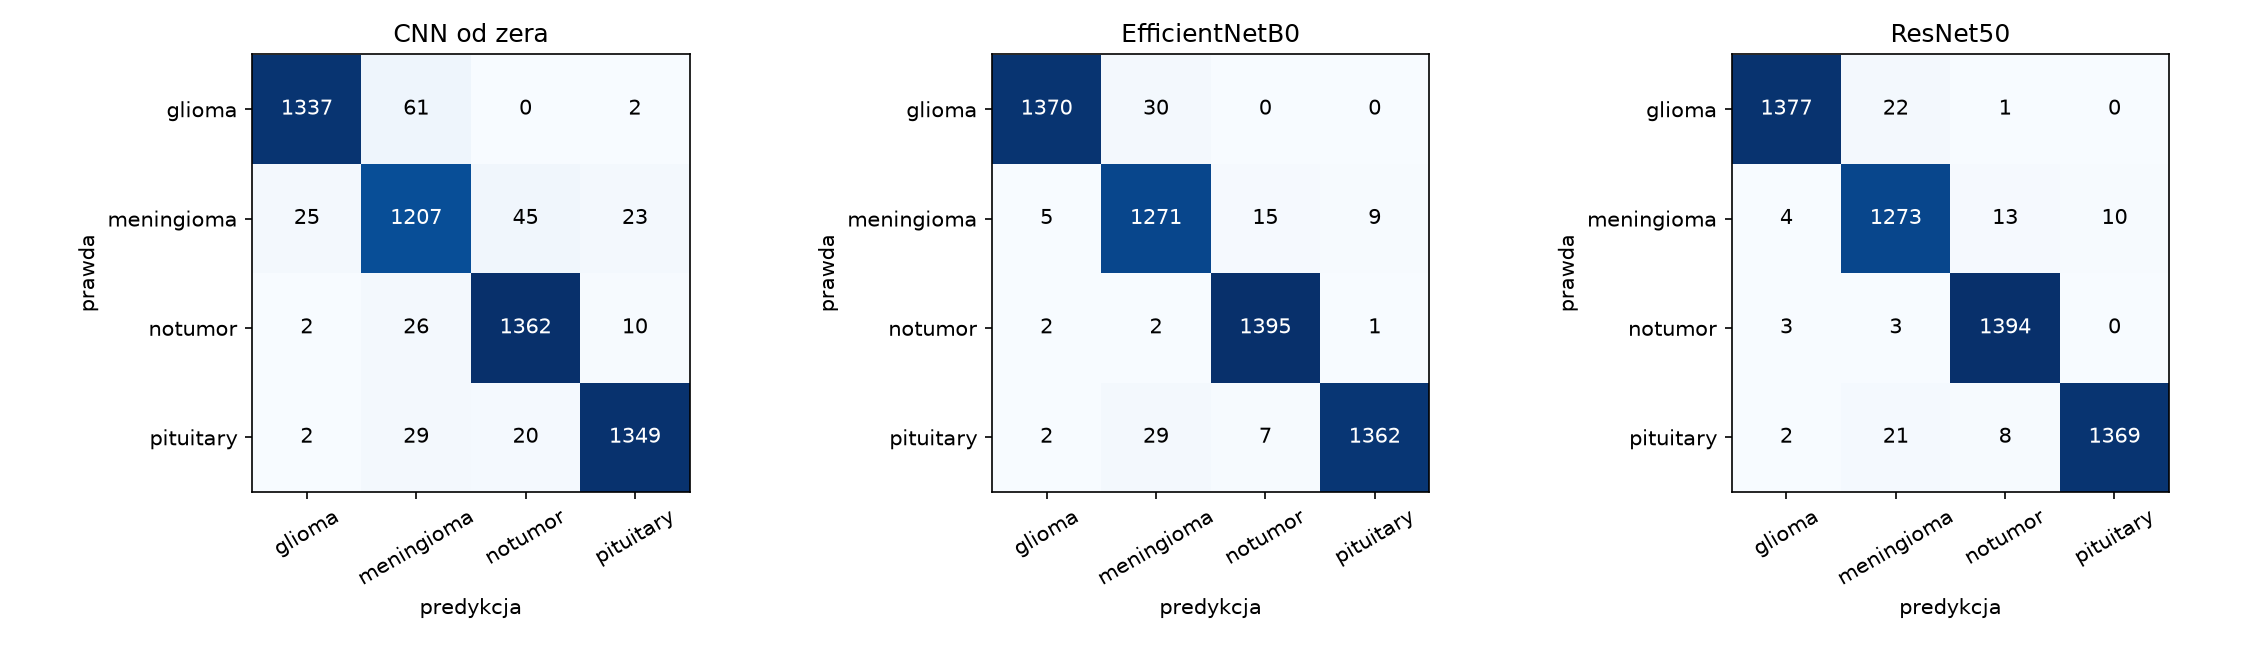
\includegraphics[width=\linewidth]{cv_macierze_oof.png}
\caption{Macierze pomyłek z predykcji out-of-fold (każdy obraz treningowy oceniony przez model,
który go nie widział).}
\label{fig:oof}
\end{figure}

\paragraph{Wyniki na zbiorze testowym} (tab.~\ref{tab:test}).
Zbiór testowy został użyty jeden raz, dla czterech modeli końcowych. Najlepszy model,
ResNet50 po strojeniu, osiąga na oryginalnym teście accuracy \accTestResTuned{}
(95\,\% CI \accCiTestResTuned{}) i macro-F1 \fTestResTuned{}. Na teście oczyszczonym
z duplikatów wyniki są wyraźnie niższe: accuracy \accDedupResTuned{} (\accCiDedupResTuned{})
i macro-F1 \fDedupResTuned{} (\fCiDedupResTuned{}). Taki sam spadek widać dla wszystkich
modeli. Część oryginalnego testu to kopie obrazów treningowych, które model ,,pamięta''.
Dlatego za miarodajny uważamy wynik na \texttt{test\_dedup}, a wynik na oryginalnym teście
podajemy tylko dla porównania z literaturą. Kolejność modeli jest taka sama jak w CV
(CNN wyraźnie najsłabsza), ale przedziały ufności EfficientNetB0 i obu wersji ResNet50
w dużej mierze się pokrywają. Strojenie nie dało więc istotnej statystycznie poprawy.

Wyniki na teście są niższe niż w walidacji krzyżowej (macro-F1 \cvFResTuned{} po strojeniu). Wyjaśnia to
analiza błędów (rozdz.~\ref{sec:bledy}): w teście są glejaki z innego źródła danych,
których w treningu nie było. Wartości per klasa (tab.~\ref{tab:klasy-test} i
\ref{tab:klasy-dedup}) pokazują, że wszystkie błędy dotyczą praktycznie jednej klasy:
\begin{itemize}
\item czułość dla glejaka wynosi tylko \sensDedupGlioma{} (\sensCiDedupGlioma{}) na \texttt{test\_dedup},
  przy swoistości \specDedupGlioma{} -- model nigdy nie nazywa glejakiem czegoś innego,
  ale co piąty glejak umyka,
\item czułość dla oponiaka, guza przysadki i klasy \texttt{notumor} jest bliska 1,
\item swoistość klasy \texttt{notumor} to \specDedupNotumor{} (\specCiDedupNotumor{}): część
  obrazów z guzem (glejaków) model uznaje za obraz bez guza. Klinicznie to najgroźniejszy błąd
  (fałszywe uspokojenie),
\item AUC dla wszystkich klas jest wysokie (glejak \aucDedupGlioma{}, pozostałe $\geq$ 0,98),
  co oznacza, że prawdopodobieństwa porządkują obrazy dość dobrze. Problem leży w progu
  decyzyjnym i w pewności modelu na obrazach spoza znanej dystrybucji.
\end{itemize}
Kalibracja (rys.~\ref{fig:kal}) jest przyzwoita (ECE \eceDedupResTuned{} na \texttt{test\_dedup}),
ale błędy na glejakach mają pewność bliską 1, więc wysoka pewność nie chroni przed pomyłką.
Na małym oczyszczonym teście (tylko \nDedupNotumor{} obrazów \texttt{notumor}) przedziały ufności są
szerokie -- dlatego je raportujemy.


\begin{table}[H]
\centering
\small
\caption{Wyniki na teście oryginalnym i oczyszczonym (w nawiasach 95\,\% przedziały ufności z bootstrapu).}
\label{tab:test}
\resizebox{\linewidth}{!}{\tabela{test}}
\end{table}

\begin{table}[H]
\centering
\small
\caption{Metryki per klasa najlepszego modelu (ResNet50 po strojeniu) na teście oryginalnym.}
\label{tab:klasy-test}
\resizebox{\linewidth}{!}{\tabela{klasy_test}}
\end{table}

\begin{table}[H]
\centering
\small
\caption{Metryki per klasa najlepszego modelu na teście oczyszczonym (\texttt{test\_dedup}).}
\label{tab:klasy-dedup}
\resizebox{\linewidth}{!}{\tabela{klasy_dedup}}
\end{table}

\begin{figure}[H]
\centering
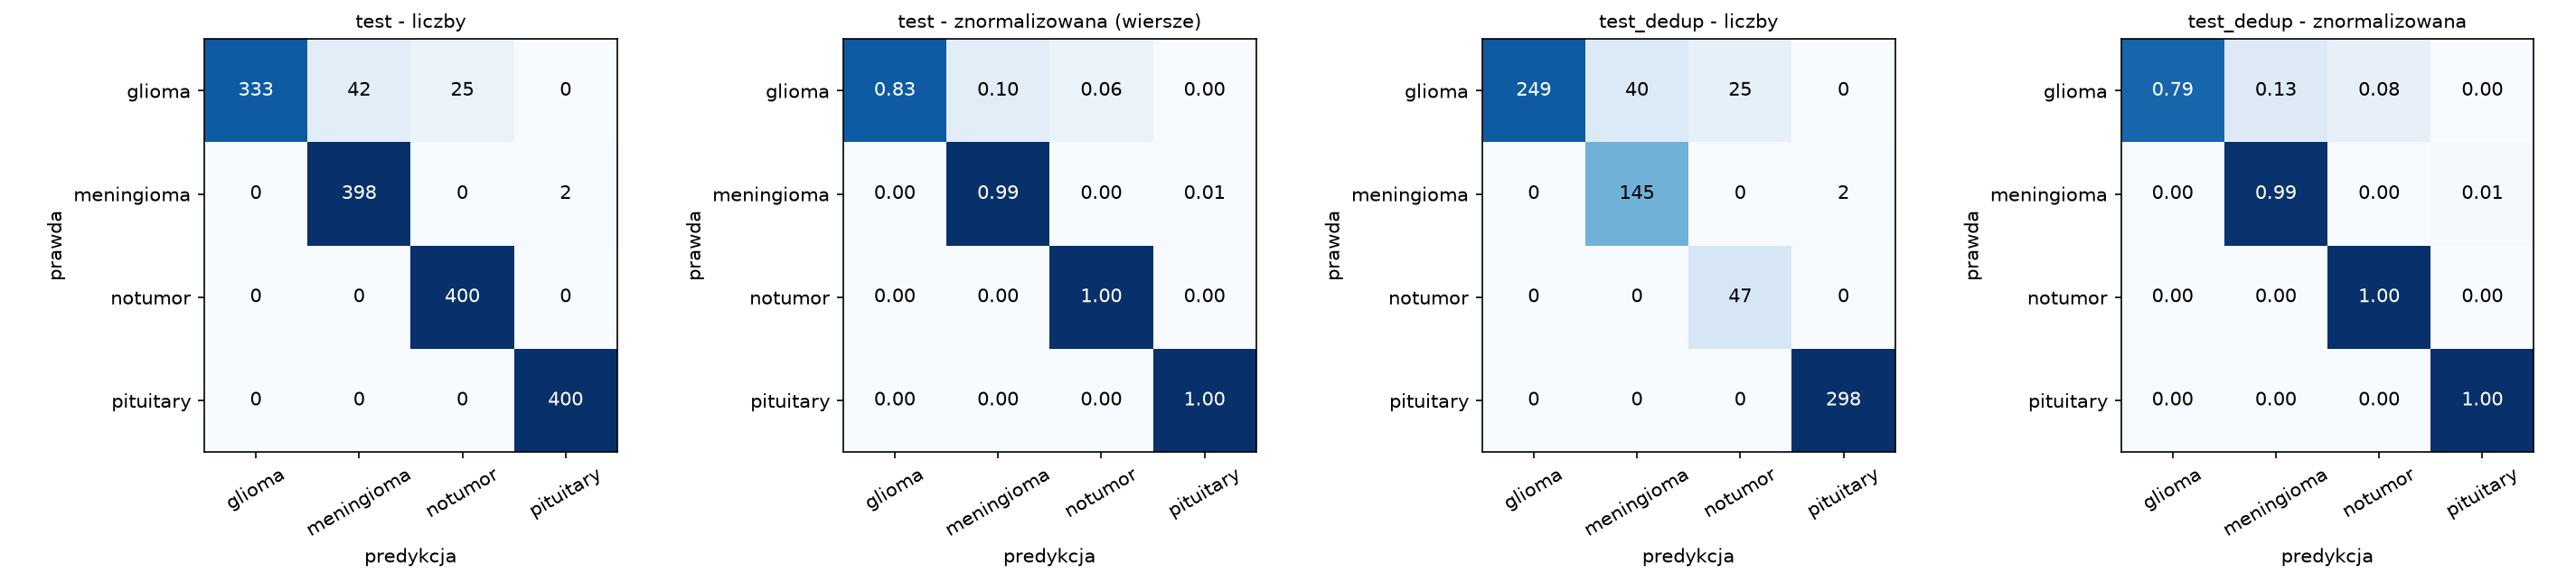
\includegraphics[width=\linewidth]{test_macierze.png}
\caption{Macierze pomyłek najlepszego modelu: test oryginalny i oczyszczony (liczby i wartości
znormalizowane wierszami, czyli czułość na przekątnej).}
\label{fig:cm}
\end{figure}

\begin{figure}[H]
\centering
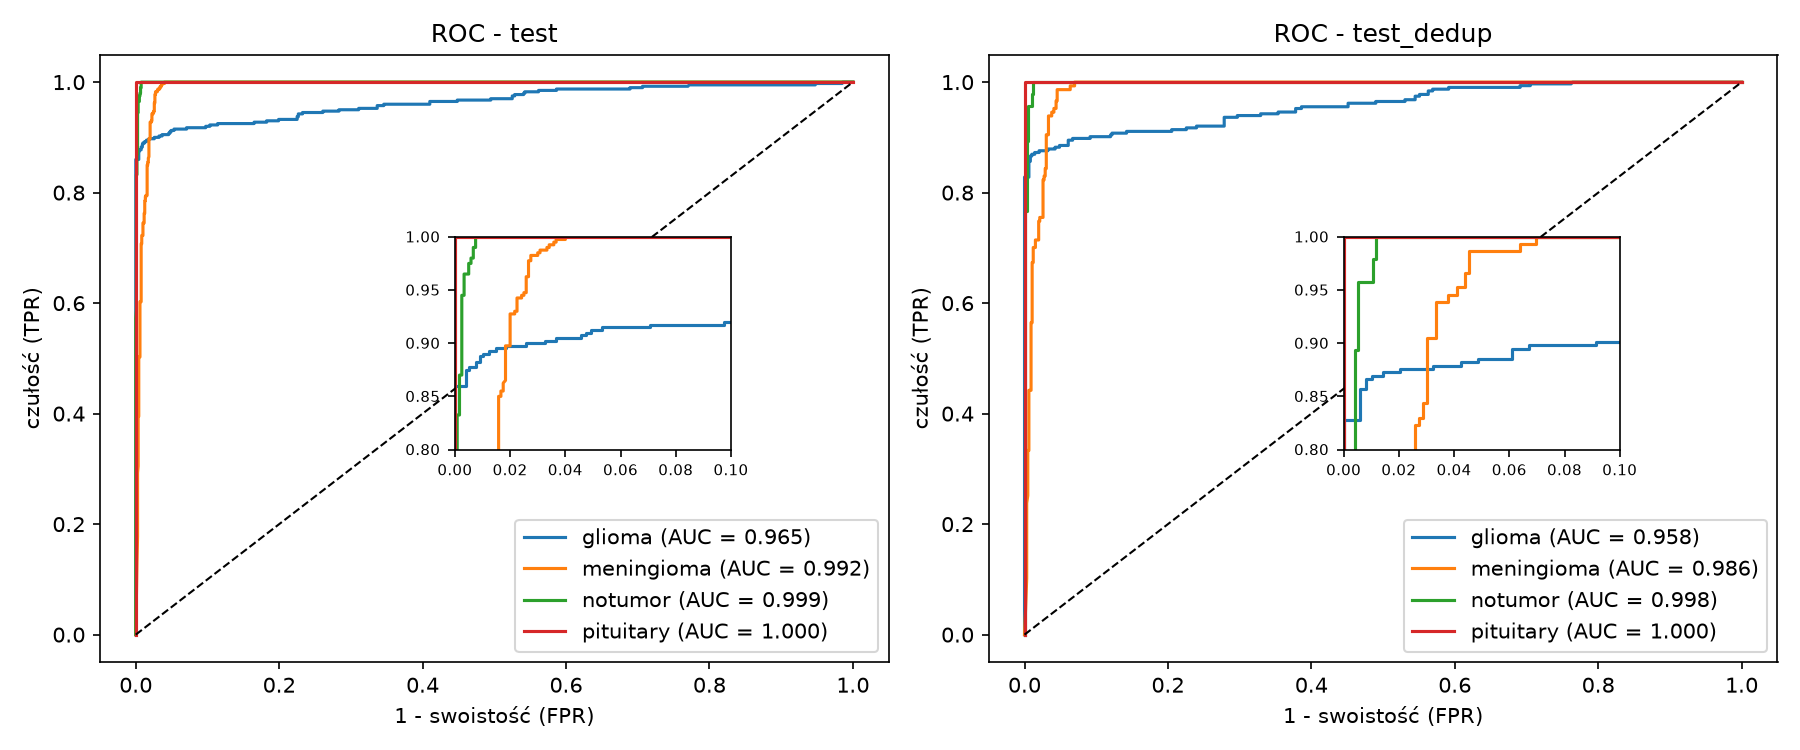
\includegraphics[width=\linewidth]{test_roc.png}
\caption{Krzywe ROC (klasa kontra reszta) najlepszego modelu; wstawki -- powiększenie lewego górnego rogu.}
\label{fig:roc}
\end{figure}

\begin{figure}[H]
\centering
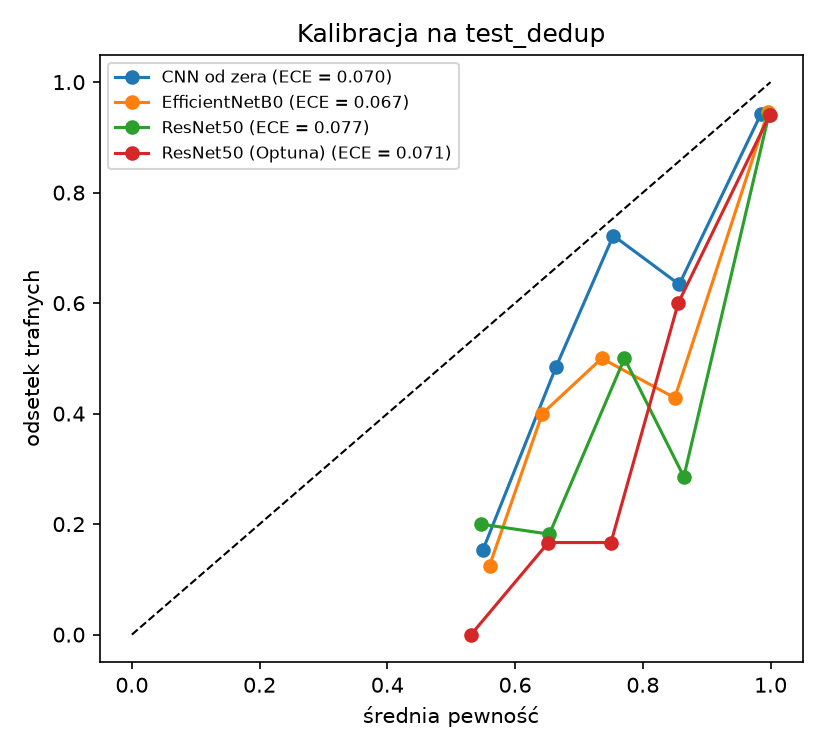
\includegraphics[width=0.55\linewidth]{test_kalibracja.png}
\caption{Wykres niezawodności (kalibracja) na teście oczyszczonym.}
\label{fig:kal}
\end{figure}

\subsection*{Dobór hiperparametrów}
Hiperparametry najlepszej architektury (ResNet50) dobrano biblioteką \textbf{Optuna}
(\texttt{src/tune.py}, notatnik \texttt{04\_tuning\_optuna.ipynb}). Jest to optymalizacja
bayesowska, a nie przeszukiwanie siatki ani losowe. Próbnik TPE (Tree-structured Parzen
Estimator) dzieli dotychczasowe próby na lepsze i gorsze, modeluje rozkład hiperparametrów
w obu grupach i proponuje konfiguracje, dla których stosunek tych rozkładów jest największy.
Słabe próby przerywa MedianPruner: po każdym foldzie porównuje średni wynik próby z medianą
wcześniejszych prób na tym samym etapie (idea Successive Halving z wykładu).

Przestrzeń poszukiwań: LR głowicy $10^{-4}$--$3\cdot10^{-3}$ (skala logarytmiczna), weight decay
$10^{-6}$--$10^{-2}$ (log.), dropout 0--0,5, batch size \{16, 32, 64\}, liczba odmrożonych
bloków szkieletu 1--\nBlocks{}. Funkcja celu to średnie macro-F1 na foldach walidacyjnych 0--2
(10 epok na próbę). Zbiór testowy nie był używany. Badanie liczy \nTrials{} prób
(\nTrialsComplete{} zakończonych, \nTrialsPruned{} przyciętych). Dodatkowo jedna próba została
przerwana przez wyłączenie komputera. Optuna zapisuje próby w bazie SQLite, więc strojenie wznowiono
i dokończono do \nTrials{} prób.

Najlepsza konfiguracja: LR $\optLr$, weight decay $\optWd$, dropout \optDropout{}, batch size
\optBatch{}, \optUnfreeze{} odmrożone bloki. Najważniejszym hiperparametrem okazał się LR
(ważność fANOVA \impLr{}), potem dropout (\impDropout{}) i weight decay (\impWd{}).

\begin{figure}[H]
\centering
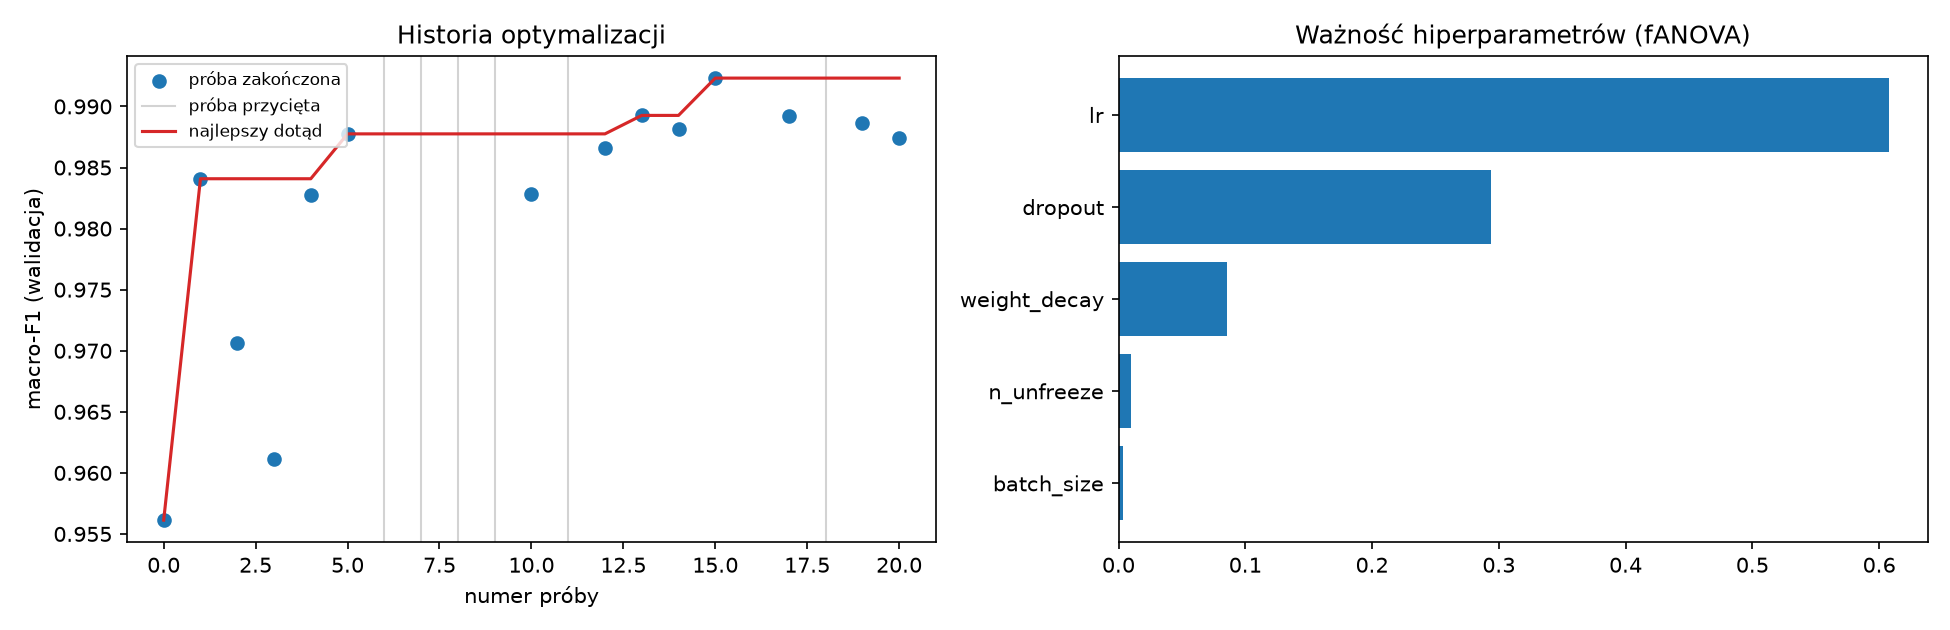
\includegraphics[width=\linewidth]{optuna.png}
\caption{Historia optymalizacji (szare linie -- próby przycięte) i ważność hiperparametrów.}
\label{fig:optuna}
\end{figure}

\paragraph{Ryzyko przeoptymalizowania na walidacji.} Najlepsza próba osiągnęła na walidacji
macro-F1 \optBest{}, ale ta liczba jest zawyżona. Wybieramy maksimum z wielu prób liczonych na
tych samych foldach, więc część przewagi to przypadek (wykład~4). W pełnej 5-krotnej walidacji
parametry po strojeniu dały \cvFResTuned{} $\pm$ \cvFsdResTuned{} wobec \cvFRes{} $\pm$ \cvFsdRes{}
dla parametrów domyślnych. Poprawa jest mniejsza niż odchylenie między foldami, a foldy 0--2
służyły do strojenia. Poprawną metodą byłaby zagnieżdżona walidacja krzyżowa, jednak jest
ok.~5 razy droższa obliczeniowo. Ostatecznym sprawdzianem był test: po strojeniu macro-F1 na
\texttt{test\_dedup} wzrosło z \fDedupRes{} do \fDedupResTuned{}, ale przedziały ufności
się pokrywają.



% ---------------------------------------------------------------- 4
\section{Interpretacja wyników i wyjaśnialność}\label{sec:xai}
\subsection*{Wyjaśnialność: Grad-CAM i mapy saliency}
Dla obrazów cechami są piksele, więc zamiast ważności cech (SHAP, permutation importance)
zastosowano metodę dedykowaną sieciom konwolucyjnym: \textbf{Grad-CAM} (wykład~5). Implementacja
własna na hookach PyTorch (\texttt{src/gradcam.py}):
\begin{enumerate}
\item zapamiętujemy aktywacje $A^k$ ostatniej warstwy konwolucyjnej (dla ResNet50: \texttt{layer4},
  2048 kanałów 7$\times$7) i gradient wyniku klasy $c$ względem nich,
\item waga kanału $\alpha_k^c$ to średni gradient w kanale $k$,
\item mapa $L^c = \mathrm{ReLU}\big(\sum_k \alpha_k^c A^k\big)$ jest skalowana do 224$\times$224
  i nakładana na obraz.
\end{enumerate}

\begin{figure}[H]
\centering
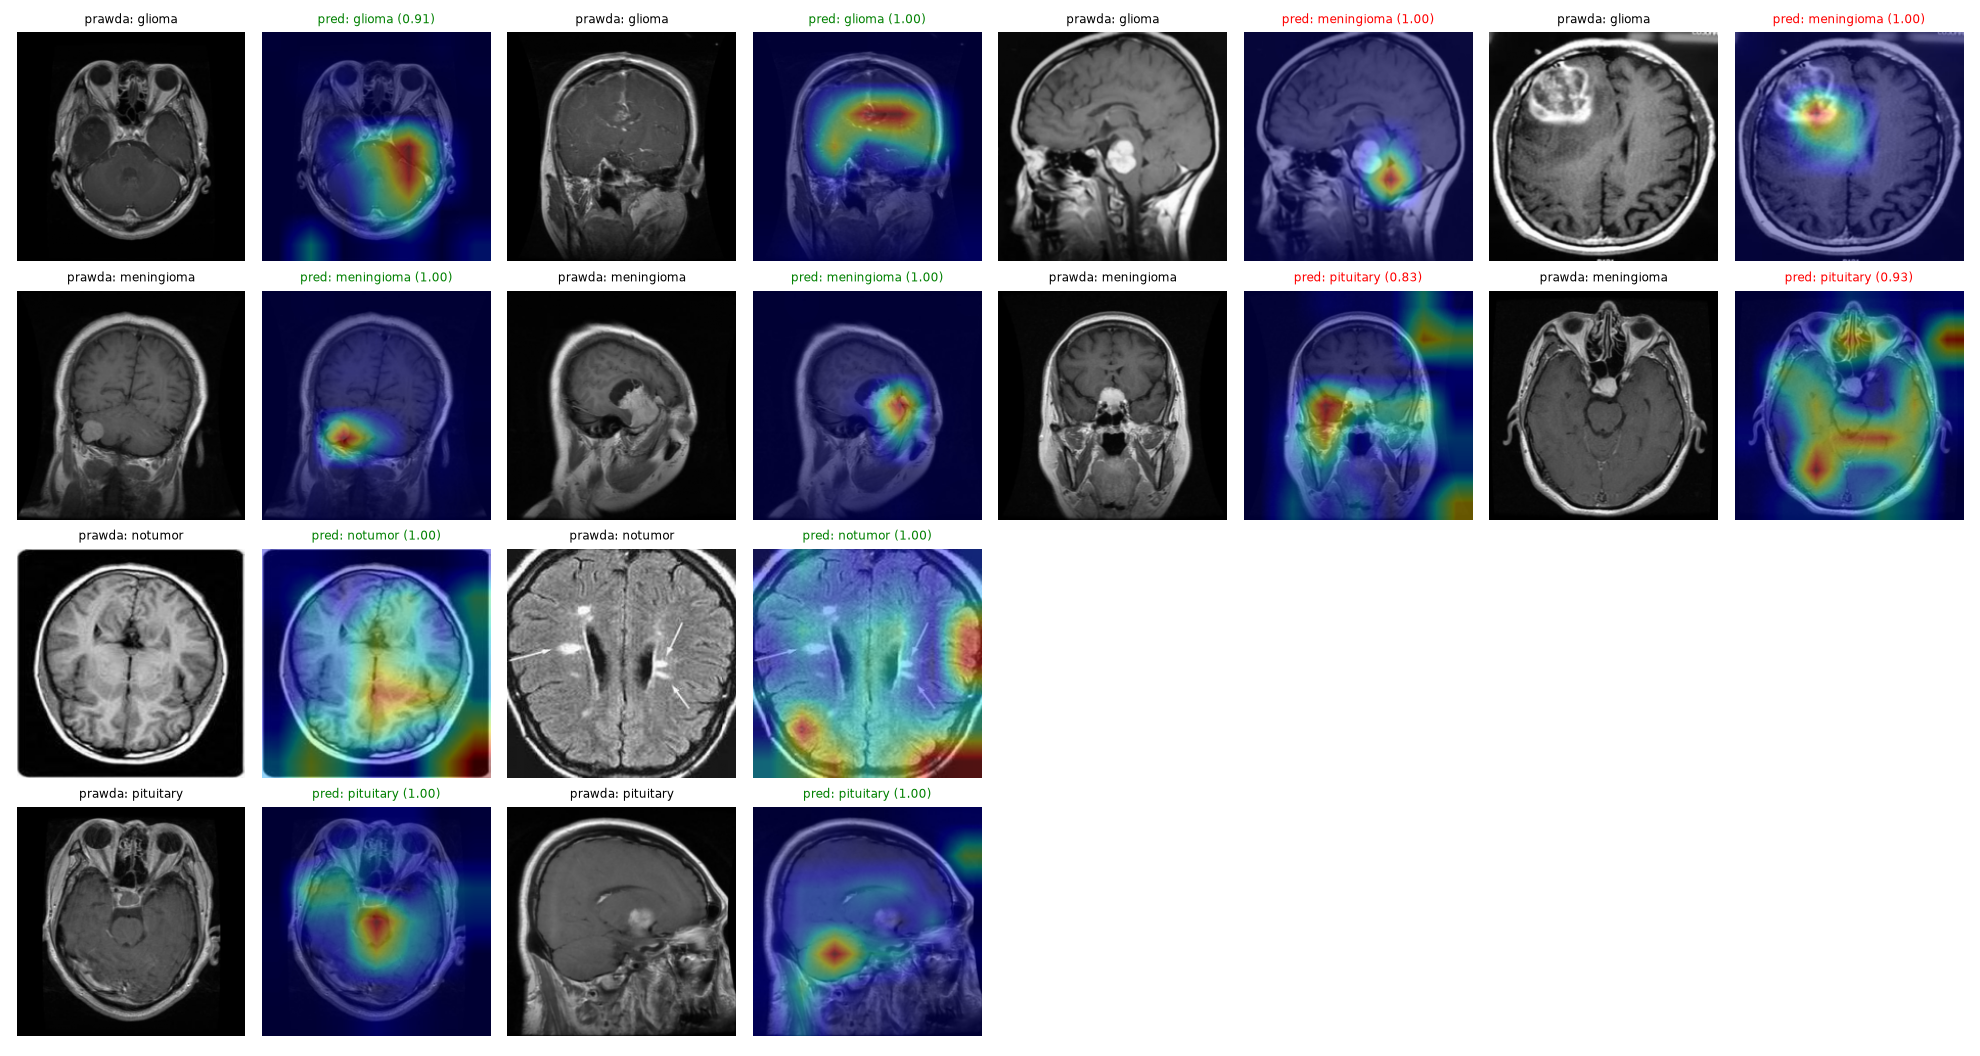
\includegraphics[width=\linewidth]{gradcam_galeria.png}
\caption{Grad-CAM dla trafnych (zielone) i błędnych (czerwone) predykcji z każdej klasy
(\texttt{test\_dedup}). Dla \texttt{notumor} i \texttt{pituitary} nie ma błędów.}
\label{fig:gradcam}
\end{figure}

Dla glejaków, oponiaków i guzów przysadki mapy w większości przypadków wskazują zmianę
nowotworową lub okolicę siodła tureckiego, czyli obszary zgodne z intuicją kliniczną
(rys.~\ref{fig:gradcam}). Dla klasy \texttt{notumor} mapa jest rozlana po całym obrazie,
także na tło i brzegi kadru. Model nie ,,sprawdza'', czy guza brak, tylko rozpoznaje ogólny
wygląd obrazu. Żeby nie opierać się na kilku wybranych obrazach (ryzyko nadinterpretacji,
wykład~5), policzono dla wszystkich obrazów \texttt{test\_dedup}, jaka część mapy leży na tle
(piksele ciemniejsze niż 20) i w pasie brzegowym (zewnętrzne 10\,\% szerokości, czyli
\borderArea{} powierzchni) -- tab.~\ref{tab:gradcam}. Dla klas z guzem na tło przypada średnio
\camBgTumor{} masy mapy, a dla \texttt{notumor} \camBgNotumor{}; na brzeg odpowiednio
\camBorderTumor{} i \camBorderNotumor{}. Mapy dla klas z guzem są więc skupione na głowie,
a dla \texttt{notumor} bliższe rozkładowi równomiernemu.

\begin{table}[H]
\centering
\caption{Gdzie leży masa mapy Grad-CAM (średnia po obrazach \texttt{test\_dedup}).}
\label{tab:gradcam}
\tabela{gradcam}
\end{table}

Dla porównania policzono najprostszą mapę saliency (moduł gradientu wyniku po pikselach,
rys.~\ref{fig:saliency}). Dla klas z guzem wskazuje podobne obszary jak Grad-CAM, ale jest
dużo bardziej zaszumiona. Dla obrazu \texttt{notumor} wyraźnie podkreśla ramkę i krawędzie
kadru, co wspiera hipotezę, że cechy techniczne obrazu (kadrowanie, źródło) wpływają na
decyzję. Metody nie są w pełni zgodne (wykład~5: niekonsekwencje technik wyjaśnialności),
a obie pokazują korelację, nie przyczynę. Traktujemy je jako wskazówkę do analizy błędów,
nie jako dowód poprawnego rozumowania modelu.

\begin{figure}[H]
\centering
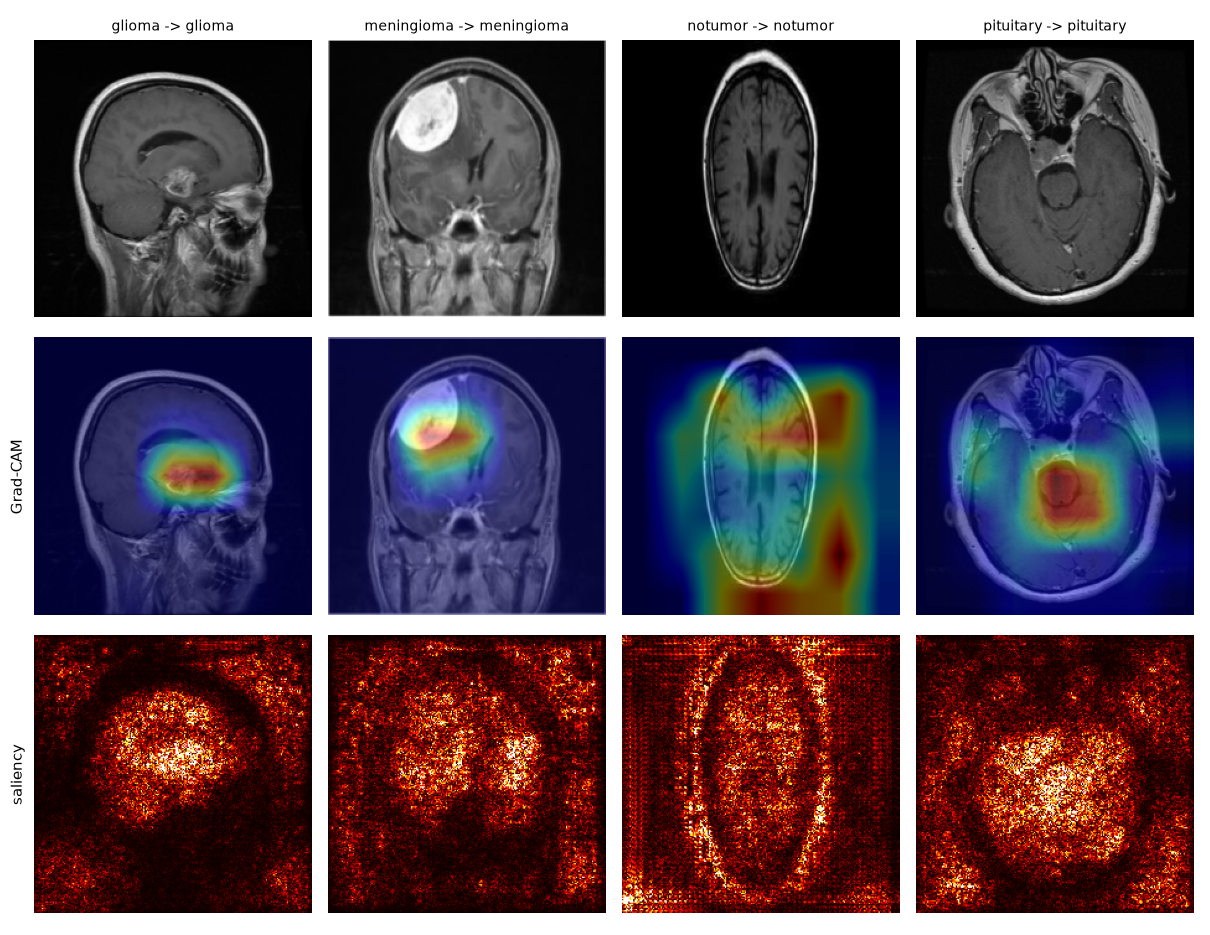
\includegraphics[width=0.75\linewidth]{gradcam_vs_saliency.png}
\caption{Ten sam obraz: Grad-CAM (środek) i mapa saliency (dół).}
\label{fig:saliency}
\end{figure}

\subsection*{Analiza błędów}\label{sec:bledy}
Najlepszy model pomylił się na \nErrTest{} z \nTestDir{} obrazów testowych, z czego
\nErrDedup{} błędów jest w \texttt{test\_dedup} (tab.~\ref{tab:bledy}). Wnioski:

\begin{table}[H]
\centering
\caption{Błędy najlepszego modelu na teście oryginalnym.}
\label{tab:bledy}
\tabela{bledy}
\end{table}

\begin{enumerate}
\item \textbf{Wyciek zawyża wynik oryginalnego testu.} Wśród obrazów, które mają w treningu
  bliźniaka tej samej klasy, odsetek błędów wynosi \errRateTwin{}, a wśród obrazów bez
  bliźniaka \errRateNoTwin{}. Dwa błędy spoza \texttt{test\_dedup} to glejaki, których
  niemal identyczny bliźniak w treningu ma etykietę \emph{oponiak}. Model ,,poprawnie
  zapamiętał'' błędną etykietę (szum etykiet z rozdz.~\ref{sec:dup}).
\item \textbf{Prawie wszystkie błędy to glejaki} (\nErrGlioma{} z \nErrTest{}):
  \nErrGliomaMeningioma{} rozpoznano jako oponiaka, a \nErrGliomaNotumor{} jako brak guza.
  Te drugie to przeoczony guz.
\item \textbf{Główna przyczyna to inne źródło obrazów (shortcut learning).} W treningu
  \emph{wszystkie} glejaki mają rozmiar 512$\times$512 (zbiór figshare, T1 po kontraście):
  glejaków o innym rozmiarze jest \gliomaOtherTrain{}. W teście jest ich \gliomaOtherTest{}
  -- pochodzą z innego źródła i często są w sekwencjach T2/FLAIR -- i model myli się na
  \gliomaOtherErr{} z nich (\gliomaOtherErrRate{}). Wśród glejaków 512$\times$512 myli się na
  \gliomaFiveErr{} z \gliomaFiveTest{}. Obrazy spoza figshare w treningu to głównie
  \texttt{notumor} (\notumorOtherTrain{}) i część oponiaków (\meningiomaOtherTrain{}), więc
  ,,nietypowy'' glejak trafia właśnie do tych klas. Model powiązał klasę ze źródłem
  i sekwencją obrazu. Przed tym ostrzegała EDA (rozdzielczość, jasność). To wyjaśnia też
  różnicę między CV a testem: w treningu nie było takich glejaków, więc walidacja krzyżowa
  nie mogła tego wykryć.
\item \textbf{Pewność nie ostrzega przed błędem.} Najbardziej pewne błędy
  (rys.~\ref{fig:bledy}) mają prawdopodobieństwo ok.~1,00. Grad-CAM pokazuje, że model
  często patrzy na sam guz, ale nadaje mu zły typ: widzi zmianę, a typ ocenia na podstawie
  wyglądu całego obrazu.
\item \textbf{Glejak a oponiak} (rys.~\ref{fig:gm}) to też para trudna z natury: oba guzy
  na pojedynczym przekroju 2D bywają podobne (wzmocnienie kontrastowe, efekt masy), a różnią
  się głównie położeniem względem opon i kształtem.
\end{enumerate}

\begin{figure}[H]
\centering
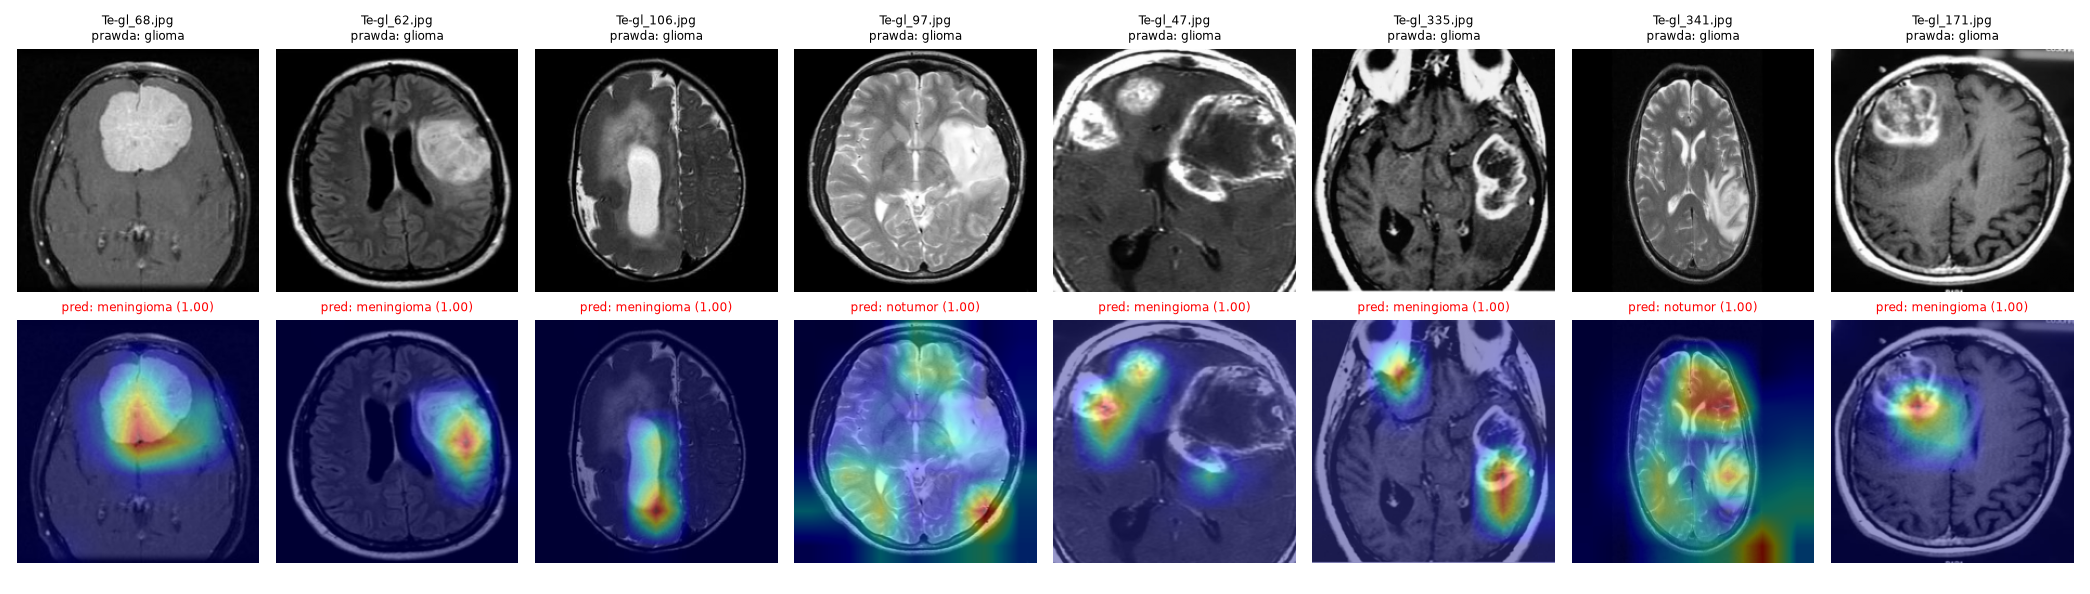
\includegraphics[width=\linewidth]{bledy_pewne.png}
\caption{Osiem najbardziej pewnych błędów najlepszego modelu z mapami Grad-CAM.}
\label{fig:bledy}
\end{figure}

\begin{figure}[H]
\centering
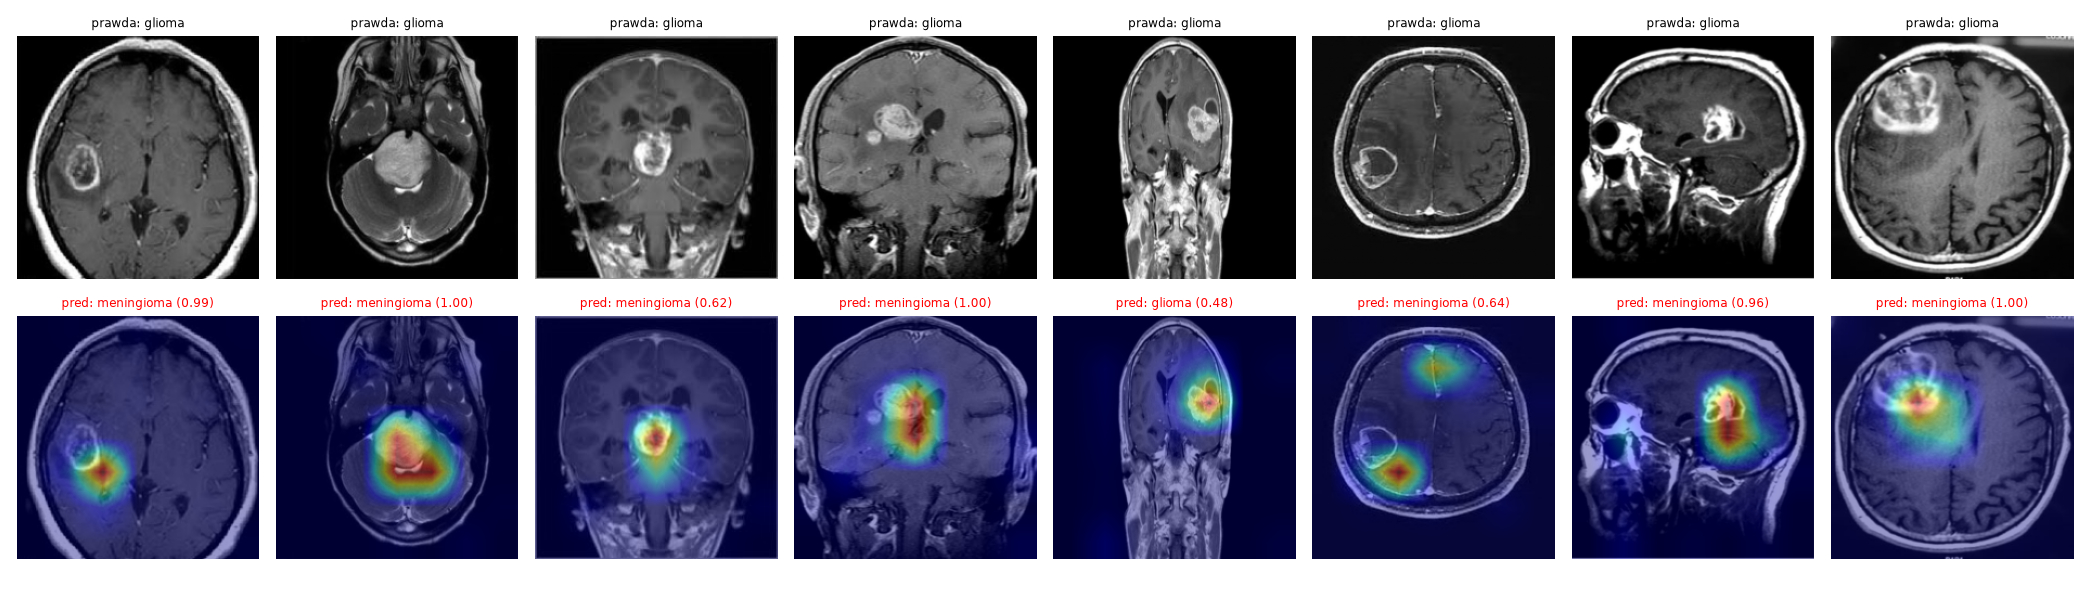
\includegraphics[width=\linewidth]{bledy_glioma_meningioma.png}
\caption{Losowe błędy glejak $\rightarrow$ oponiak.}
\label{fig:gm}
\end{figure}


% ---------------------------------------------------------------- 5
\section{Implementacja}
\subsection*{Interfejs użytkownika}
Przygotowano prosty interfejs w bibliotece Streamlit (\texttt{app.py}, uruchomienie:
\texttt{streamlit run app.py}). Użytkownik wybiera model (domyślnie ResNet50 po strojeniu),
wgrywa obraz MRI (JPG/PNG) lub wybiera obraz z katalogu \texttt{Testing}, a aplikacja pokazuje:
\begin{itemize}
\item przewidzianą klasę i jej prawdopodobieństwo,
\item obraz wejściowy po przetworzeniu (skala szarości, 224$\times$224) obok mapy Grad-CAM,
\item wykres prawdopodobieństw wszystkich czterech klas.
\end{itemize}
Na górze strony jest wyraźne zastrzeżenie, że to narzędzie edukacyjne, a nie wyrób medyczny.
Pod mapą jest też informacja, że Grad-CAM nie jest segmentacją guza. Interfejs korzysta z tych
samych funkcji co notatniki (\texttt{load\_image}, \texttt{grad\_cam}), więc przetwarzanie
obrazu jest identyczne jak podczas ewaluacji. Rys.~\ref{fig:gui} pokazuje poprawną predykcję
guza przysadki oraz typowy błąd: glejak w sekwencji FLAIR rozpoznany z pełną pewnością jako
oponiak, mimo że mapa wskazuje guz.

\begin{figure}[H]
\centering
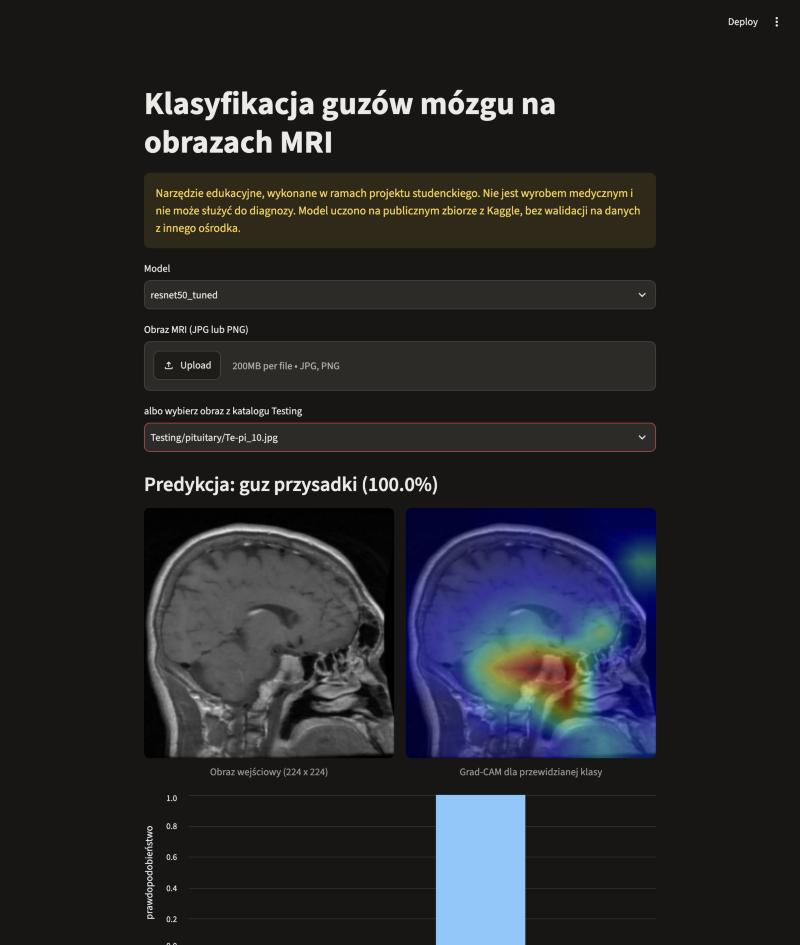
\includegraphics[width=0.48\linewidth]{gui_przysadka.jpg}\hfill
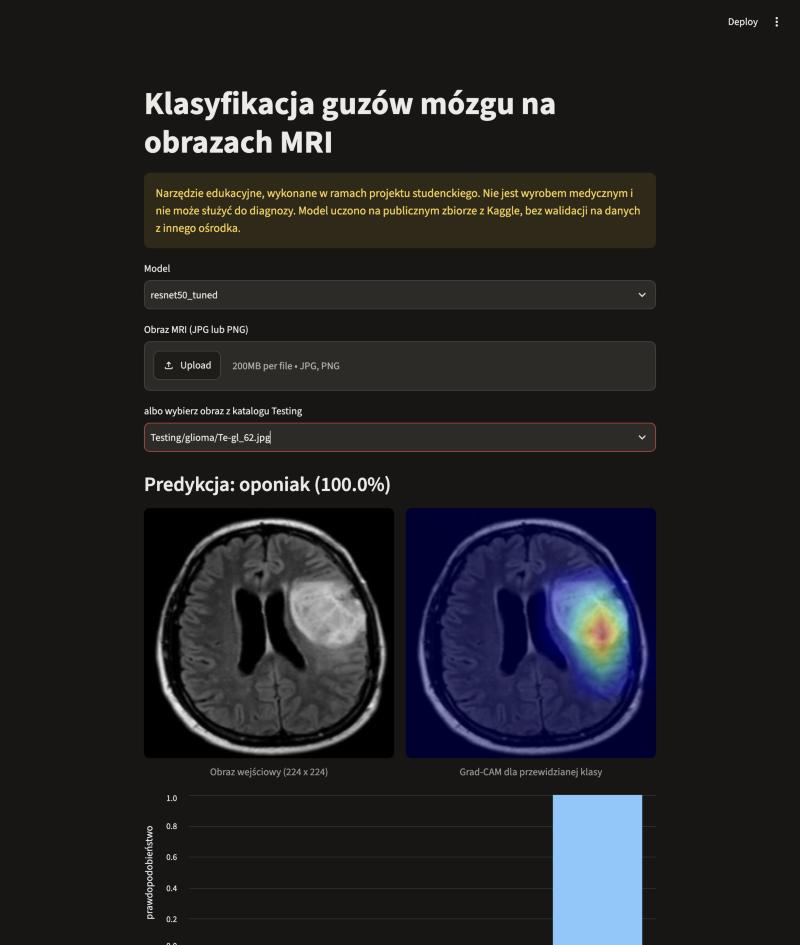
\includegraphics[width=0.48\linewidth]{gui_glejak_blad.jpg}
\caption{Interfejs Streamlit: poprawna predykcja guza przysadki (po lewej) i błędna predykcja
glejaka z innego źródła danych (po prawej).}
\label{fig:gui}
\end{figure}


% ---------------------------------------------------------------- 6
\section{Podsumowanie}
\subsection*{Wnioski}
\begin{itemize}
\item Transfer wiedzy z ImageNet daje wyraźnie lepsze wyniki niż sieć uczona od zera
  (macro-F1 w CV \cvFRes{} i \cvFEff{} wobec \cvFCnn{}). ResNet50 i EfficientNetB0 są
  praktycznie równorzędne, przy czym EfficientNetB0 jest ok.~6 razy mniejszy. Strojenie
  Optuną poprawiło wyniki nieznacznie, w granicach niepewności.
\item Najlepszy model (ResNet50 po strojeniu) osiąga na oryginalnym teście accuracy
  \accTestResTuned{}, a na teście oczyszczonym z duplikatów \accDedupResTuned{}
  (macro-F1 \fDedupResTuned{}). Różnica pokazuje, jak bardzo duplikaty między treningiem
  i testem zawyżają wyniki publikowane dla tego zbioru.
\item Model bardzo dobrze rozpoznaje guzy przysadki, oponiaki i obrazy bez guza, ale gubi
  glejaki pochodzące z innego źródła niż dane treningowe (czułość dla glejaka
  \sensDedupGlioma{}). Część z nich uznaje za obraz bez guza. Analiza błędów i Grad-CAM
  wskazują, że model częściowo nauczył się rozpoznawać \emph{źródło i sekwencję} obrazu
  zamiast cech guza.
\item W praktyce klinicznej taki model mógłby co najwyżej wspierać wstępne sortowanie badań
  (triage), z wynikiem zawsze weryfikowanym przez radiologa. W obecnej postaci nie nadaje się
  do użycia: przeoczenie co piątego glejaka z nowego źródła jest nieakceptowalne.
\end{itemize}

\subsection*{Problemy i ograniczenia}
\begin{itemize}
\item \textbf{Brak identyfikatora pacjenta.} Nie da się zrobić podziału per pacjent.
  Grupowanie niemal-duplikatów pHash jest tylko przybliżeniem: sąsiednie przekroje tego
  samego pacjenta mogą różnić się bardziej niż próg.
\item \textbf{Zbiór złożony z kilku źródeł}, w których klasy są nierówno reprezentowane
  (glejaki w treningu tylko z jednego źródła, obrazy bez guza głównie z innych). To główna
  przyczyna błędów. Do tego sztuczny balans (kopie \texttt{aug}) i szum etykiet
  (\nPairsConflict{} par niemal identycznych obrazów z różnymi etykietami).
\item \textbf{Pojedyncze przekroje 2D} zamiast całych badań 3D i różnych sekwencji tego samego
  pacjenta; radiolog ocenia całe badanie.
\item \textbf{Brak walidacji zewnętrznej} (inny szpital, inny skaner). Oczyszczony test pochodzi
  z tych samych źródeł co trening i jest mały (\nTestDedup{} obrazów, w tym tylko \nDedupNotumor{}
  bez guza), stąd szerokie przedziały ufności.
\item \textbf{Strojenie} na tych samych foldach co ocena CV (brak zagnieżdżonej walidacji).
\item Rozdzielczość 224$\times$224 może ukrywać drobne zmiany. Wyjaśnienia Grad-CAM mają niską
  rozdzielczość (7$\times$7) i pokazują korelacje, nie przyczyny.
\end{itemize}

\subsection*{Aspekty etyczne i prawne}
Obrazy medyczne to dane szczególnej kategorii (art.~9 RODO). Ich użycie wymaga podstawy
prawnej i anonimizacji, a pacjent ma prawo do informacji o zautomatyzowanym przetwarzaniu
i do wyjaśnienia decyzji (art.~22). Uprzedzenia ukryte w danych -- tu powiązanie klasy ze
źródłem obrazu -- nie są widoczne w samych metrykach i mogą prowadzić do systematycznie
gorszej diagnozy dla pacjentów badanych w innych ośrodkach. Odpowiedzialność za decyzję
zawsze ponosi lekarz.

\subsection*{Możliwości rozwoju}
\begin{itemize}
\item Dane: zbiory z identyfikatorem pacjenta i wieloma ośrodkami (np. BraTS -- badania 3D
  z wieloma sekwencjami), walidacja na zewnętrznym zbiorze, glejaki z różnych źródeł w treningu.
\item Walidacja grupowa według źródła (leave-one-source-out), żeby wprost mierzyć
  przenoszenie się modelu na nowy ośrodek.
\item Normalizacja intensywności per obraz (np. z-score w obrębie mózgu), usunięcie ramek
  i znaczników, wycinanie samego mózgu -- żeby utrudnić uczenie się skrótów.
\item Segmentacja guza (np. U-Net) zamiast samej klasyfikacji, modele 3D.
\item Progi decyzyjne dobrane pod wysoką czułość klas nowotworowych, kalibracja
  (temperature scaling) i wykrywanie obrazów spoza znanej dystrybucji (odmowa odpowiedzi
  przy niepewności).
\end{itemize}


% ---------------------------------------------------------------- 7
\section{Załączniki}\label{sec:zal}
\begin{itemize}
\item Repozytorium: \url{https://github.com/balicz3k/BrainTumorClassification}
\item Notatniki z wynikami: \texttt{notebooks/01\_eda.ipynb} -- \texttt{05\_ewaluacja\_wyjasnialnosc.ipynb}.
\item Kod: \texttt{src/} (dane, modele, trening, strojenie, metryki, Grad-CAM), GUI: \texttt{app.py}.
\item Surowe wyniki: \texttt{out/metrics/} (JSON i CSV), wykresy: \texttt{out/figures/}.
\item Instrukcja odtworzenia wyników: \texttt{README.md}.
\end{itemize}

\end{document}
